%-------------------------------------------------------------------------------
% Copyright (c) 2015-2016 University of Luxembourg.
% All rights reserved. This program and the accompanying materials
% are made available under the terms of the Eclipse Public License v1.0
% which accompanies this distribution, and is available at
% http://www.eclipse.org/legal/epl-v10.html
% 
% Contributors:
%     Alfredo Capozucca - initial API and implementation
%     Benoit Ries - minor updates
%     Nicolas Guelfi - most content from messirbook
%-------------------------------------------------------------------------------
%%%%%%%%%%%%%%%%%%%%%%%%%%%%%%%%%%%%%%%%%%%%%%%%%%
\PassOptionsToPackage{usenames,svgnames,table}{xcolor}
\documentclass[graybox,envcountchap,sectrefs]{./../lu.uni.lassy.excalibur.standard.report.libraries/styles/svmono}  
%%%%%%%%%%%%%%%%%%%%%%%%%%%%%%%%%%%%%%%%%%%%%%%%%%
%%% DO NOT CHANGE THE ORDER
\usepackage{./../lu.uni.lassy.excalibur.standard.report.libraries/styles/style-messir-common}
\usepackage{./../lu.uni.lassy.excalibur.standard.report.libraries/styles/style-messir-report-post}
\usepackage{breakurl}
\usepackage{graphicx}
\usepackage{hyperref}
\usepackage{xcolor}
%--------------------------------------------
  \newenvironment{Tab}[1]%
{\begin{list}{}
         {\setlength{\leftmargin}{#1}}
         \item[]
}
{\end{list}}
% DOCUMENT BEGIN
%--------------------------------------------
\begin{document}
%-------------------------------------------------------------------------------
\newgeometry{textwidth=17cm,textheight=23.7cm} 
 
\definecolor{lightgray}{RGB}{201,201,201}
\definecolor{lightred}{RGB}{250,112,97}
\definecolor{lightgreen}{RGB}{179,250,140}

\definecolor{msrtextcl}{RGB}{0,0,0}
\definecolor{msrkeycl}{RGB}{127,0,85}
\definecolor{msrcmtcl}{RGB}{201,201,201}
\definecolor{keywordcolor}{RGB}{30,144,255}

\definecolor{aqua_blue}{RGB}{0,139,145}
\definecolor{dark_green}{RGB}{0,128,0}
\definecolor{dark_blue}{RGB}{45,45,138}

\definecolor{msrcolor01}{rgb}{0.96,0.59,0.48}
\definecolor{msrcolor02}{rgb}{1.00,0.97,0.60}
\definecolor{msrcolor03}{rgb}{0.51,0.79,0.61}
\definecolor{msrcolor04}{rgb}{0.43,0.81,0.96}
\definecolor{msrcolor05}{rgb}{0.52,0.58,0.79}
\definecolor{msrcolor06}{rgb}{0.96,0.61,0.76}
\definecolor{msrcolor07}{rgb}{0.98,0.68,0.51}
\definecolor{msrcolor08}{rgb}{0.77,0.88,0.61}
\definecolor{msrcolor09}{rgb}{0.49,0.66,0.85}
\definecolor{msrcolor10}{rgb}{0.96,0.60,0.62}
\definecolor{msrcolor11}{rgb}{0.64,0.83,0.61}
\definecolor{msrcolor12}{rgb}{0.63,0.53,0.75}
\definecolor{msrcolor13}{rgb}{0.99,0.78,0.54}
\definecolor{msrcolor14}{rgb}{0.53,0.51,0.74}
\definecolor{msrcolor15}{rgb}{0.48,0.80,0.79}
\definecolor{msrcolor16}{rgb}{0.74,0.55,0.75}
\definecolor{msrcolor17}{rgb}{0.90,0.79,0.08}
\definecolor{msrcolor18}{rgb}{1.00,1.00,0.00}
\definecolor{msrcolor19}{rgb}{1.00,0.00,0.50}

\definecolor{sepcolor000000}{rgb}{0, 0, 0}
\definecolor{sepcolor101010}{rgb}{0.10, 0.10, 0.10}
\definecolor{sepcolor202020}{rgb}{0.20, 0.20, 0.20}
\definecolor{sepcolor303030}{rgb}{0.30, 0.30, 0.30}
\definecolor{sepcolor404040}{rgb}{0.10, 0.10, 0.10}
\definecolor{sepcolor505050}{rgb}{0,1,.5}
\definecolor{sepcolor907908}{rgb}{0,1,.5}

\definecolor{sepregioncolor01}{rgb}{0.00,0.66,0.00}
\definecolor{sepregioncolor02}{rgb}{1.00,1.00,0.00}
\definecolor{sepregioncolor03}{rgb}{1.00,0.97,0.60}
\definecolor{sepregioncolor04}{rgb}{0.64,0.83,0.61}
\definecolor{sepregioncolor05}{rgb}{0.95,0.36,0.00}
\definecolor{sepregioncolor06}{rgb}{0.90,0.79,0.08}
\definecolor{sepregioncolor07}{rgb}{0.63,0.53,0.75}
\definecolor{sepregioncolor08}{rgb}{0.99,0.78,0.54}
\definecolor{sepregioncolor09}{rgb}{0.96,0.61,0.76}
\definecolor{sepregioncolor10}{rgb}{1.00,0.00,0.50}

\colorlet{msrcolorbrown}{red!40!black!80}


% Messir General
%----------------------------------------------------------

% quotePosition + quoteWidth + quotefillColor + quoteElement + quotedElement + allImageScale
\newcommand{\msrcallouted}[6]{
\scalebox{#1}{\parbox{\linewidth}{
  \begin{tikzpicture}
      \node [rectangle callout,callout relative pointer={#4},text width=#5,fill=#6,rounded corners] (tmpcall) at (0,0) {#3};
      \node at (tmpcall.pointer){#2};
  \end{tikzpicture}
}}
}

% Vresion wihtout scaling the quoted text
\pgfkeys{%
    /calloutquote/.cd,
    width/.code                   =  {\def\calloutquotewidth{#1}},
    position/.code                =  {\def\calloutquotepos{#1}}, 
    author/.code                  =  {\def\calloutquoteauthor{#1}},
    /calloutquote/.unknown/.code   =  {\let\searchname=\pgfkeyscurrentname
                                 \pgfkeysalso{\searchname/.try=#1,
    /tikz/\searchname/.retry=#1},\pgfkeysalso{\searchname/.try=#1,
                                  /pgf/\searchname/.retry=#1}}
                            }  

\newcommand\calloutquote[2][]{%
  \pgfqkeys{/calloutquote}{#1}
  \node [rectangle callout,callout relative pointer={\calloutquotepos},text width=\calloutquotewidth,/calloutquote/.cd,#1] (tmpcall) at (0,0) {#2};
  \node at (tmpcall.pointer){\calloutquoteauthor};    
}  
%----------------------------------------------------------
\newcommand{\msrTalkRD}[6]{
\freeblock{5}{#1}{#2}{
\begin{figure}
  \centering
  \includegraphics[width=#5]{images/various/descartes.pdf} 
\end{figure}
}
\freeblock{5}{#3}{#4}{
\scriptsize
\textit{#6}
}
}
\newcommand{\msrTalkGB}[6]{
\freeblock{5}{#1}{#2}{
\begin{figure}
  \centering
  \includegraphics[width=#5]{images/various/graham-bell.pdf} 
\end{figure}
}
\freeblock{5}{#3}{#4}{
\scriptsize
\textit{#6}
}
}
%----------------------------------------------------------

\newcommand{\msrQuestionSlide}[1]{
\begin{frame}[fragile]
\freeblock{5}{1}{4}{
\begin{figure}
  \centering
  \includegraphics[width=3cm]{images/various/3d-man-question-sit.pdf}
\end{figure}
}
\freeblock{10}{5}{3}{
\Large
\msrtxtclb{red}{\textit{#1}}
}
\end{frame}
}

%%%%%%%%%%%%%%%%%%%%%%%%%%%%%%%%%%%%%%%%%%%%%%%%%%%%%%%%%%
%%%%%%%%%%%%%%%%%%%%%%%%%%%%%%%%%%%%%%%%%%%%%%%%%%
%%% AUDIO
%%%%%%%%%%%%%%%%%%%%%%%%%%%%%%%%%%%%%%%%%%%%%%%%%%

\DeclareRobustCommand{\MyIncludeMedia}[5]{%
\addmediapath{#1}
\includemedia[
  flashvars={source=#2%
  &hideBar=true%
  &autoPlay=#3%
  },
  activate=pagevisible,
  noplaybutton,
  addresource=#2,
  transparent,
  passcontext
]{\includegraphics[width=.8cm]{#4}}{APlayer.swf}%
}

\DeclareRobustCommand{\slidesAudioModeChange}[1]
{\renewcommand{\slidesAudioMode}{#1}}

\DeclareRobustCommand{\slidesAudioHelp}{%
\IfSubStr{\slidesAudioMode}%
{remove}%
{}
{%
\pdfcomment[icon=Help,color=blue!10,open=false,subject={standard 14 fonts}]{Right clic on flag to have options !\\
Audio only available with Acrobat\ldots}%
}
}


\DeclareRobustCommand{\MyAudioButton}[3]{%
\IfSubStr{\slidesAudioMode}%
{remove}%
{}
{%
\IfSubStr{#1}{pause}{\def\MyAutoPlayMode{false}}{}%
\IfSubStr{#1}{\slidesAudioMode}{\def\MyAutoPlayMode{true}}{\def\MyAutoPlayMode{false}}%
\IfSubStr{#1}%
{fr}%
{\def\MyAudioIconPath{./../MessirSlides/images/various/flag-audio-FR.pdf}}{}%
\IfSubStr{#1}%
{en}%
{\def\MyAudioIconPath{./../MessirSlides/images/various/flag-audio-EN.pdf}}{}%
\IfSubStr{#1}%
{de}%
{\def\MyAudioIconPath{./../MessirSlides/images/various/flag-audio-DE.pdf}}{}%
\IfSubStr{#1}%
{lu}%
{\def\MyAudioIconPath{./../MessirSlides/images/various/flag-audio-LU.pdf}}{}%
\MyIncludeMedia{#2}{#3}{\MyAutoPlayMode}{\MyAudioIconPath}{#1}%
}
}
\makeatletter % we need to use kernel commands
\newcommand{\MyAudioBegin}{%
\begin{flushright}%
\setstretch{.3}
\@MyAudioOne%
}
\newcommand\@MyAudioOne{\@ifnextchar\stopaudio{\@MyAudioEnd}{\@MyAudioTwo}}

\newcommand\@MyAudioTwo[3]{%
\hspace*{-0.1cm}\@MyAudioThree{#1}{#2}{#3}%
\@MyAudioOne% restart the recursion
}
\newcommand\@MyAudioThree[3]{%
\MyAudioButton{#1}%
{#2}%
{#3}%
}
\newcommand\@MyAudioEnd[1]{% The argument is \stopaudio
\end{flushright}%
}
\makeatother

%%%%%%%%%%%%%%%%%%%%%%%%%%%%%%%%%%%%%%%%%%%%%%%%%%

\DeclareRobustCommand{\msrfigure}[4]{
\begin{figure}[!htbp]
\begin{center}
\scalebox{#1}{
\centering
{\begin{minipage}[c]{\linewidth}
\centering
#2
\end{minipage}
}}
\end{center}
\ifthenelse{\equal{#4}{}}
             {}
             {\caption{#4}}
\label{#3}
\end{figure}
}

\newcommand{\semitransp}[2][30]{\color{fg!#1}#2}
\newcommand*{\msrtechfont}{\fontfamily{ptm}\selectfont}

\DeclareRobustCommand{\msruml}{{\msrtechfont UML}~}
\DeclareRobustCommand{\msrocl}{{\msrtechfont OCL}~}
\DeclareRobustCommand{\msromg}{{\msrtechfont OMG}~}
\DeclareRobustCommand{\msrxtext}{{\msrtechfont Xtext}~}
\DeclareRobustCommand{\msremf}{{\msrtechfont EMF}~}
\DeclareRobustCommand{\msrcm}{\msrcode{{Concept Model}}~}

\DeclareRobustCommand{\msrapache}{{\msrtechfont Apache}~}
\DeclareRobustCommand{\msratlassian}{{\msrtechfont Atlassian}~}
\DeclareRobustCommand{\msrbamboo}{{\msrtechfont Bamboo}~}
\DeclareRobustCommand{\msrconfluence}{{\msrtechfont Confluence}~}
\DeclareRobustCommand{\msreclemma}{{\msrtechfont EclEmma}~}
\DeclareRobustCommand{\msreclipse}{{\msrtechfont Eclipse}~}
\DeclareRobustCommand{\msrsql}{{\msrtechfont SQL}~}
\DeclareRobustCommand{\msrjava}{{\msrtechfont Java}~}
\DeclareRobustCommand{\msrjavafx}{{\msrtechfont JavaFx}~}
\DeclareRobustCommand{\msrjira}{{\msrtechfont JIRA}~}
\DeclareRobustCommand{\msrjunit}{{\msrtechfont JUnit}~}
\DeclareRobustCommand{\msrlatex}{{\msrtechfont Latex}~}
\DeclareRobustCommand{\msrmaven}{{\msrtechfont Maven}~}
\DeclareRobustCommand{\msrmysql}{{\msrtechfont MySQL}~}
\DeclareRobustCommand{\msrocl}{{\msrtechfont OCL}~}
\DeclareRobustCommand{\msrpdf}{{\msrtechfont PDF}~} 
\DeclareRobustCommand{\msrsirius}{{\msrtechfont Sirius}~} 
\DeclareRobustCommand{\msrsvn}{{\msrtechfont SubVersioN}~}
\DeclareRobustCommand{\msrswtbot}{{\msrtechfont SWTbot}~}
\DeclareRobustCommand{\msrxtext}{{\msrtechfont Xtext}~} 

 
\DeclareRobustCommand{\msrmessirmeth}{{\msrmessir}~methodology~}
\newcommand{\msrglsstyle}[1]{\emph{#1}}
\DeclareRobustCommand{\msrucname}[1]{\msrcode{\underline{#1}}}

% Verify macro since creates .toc errors
%\DeclareRobustCommand{\msrcode}[1]{{\normalfont\fontfamily{pcrr}\selectfont #1}}
%\DeclareRobustCommand{\msrcode}[1]{{\normalfont\fontfamily{cmvtt}\selectfont #1}}
\DeclareRobustCommand{\msrcode}[1]{{\protect\ \ttfamily \hyphenchar\font=`\- #1}}

% Messir Lexique
\DeclareRobustCommand{\msrbool}{\msrcode{{\emph Boolean}}~}
\DeclareRobustCommand{\msrint}{\msrcode{{\emph Integer}}~}
\DeclareRobustCommand{\msrreal}{\msrcode{{\emph Real}}~}
\DeclareRobustCommand{\msrstring}{\msrcode{{\emph String}}~}
\DeclareRobustCommand{\msrenum}{\msrcode{{\emph enumeration}}~}
\DeclareRobustCommand{\msrenums}{\msrcode{{\emph enumerations}}~}

% Messir Analysis
\DeclareRobustCommand{\msrsysop}{\emph{system operation}}
\DeclareRobustCommand{\msrsysops}{\emph{system operations}}
\DeclareRobustCommand{\msrsysintpro}{\emph{system interaction protocol}}
\DeclareRobustCommand{\msrbhvmd}{\emph{system operation}}

\newcommand{\msrt}[1]{\textuncl{#1}~}

\DeclareRobustCommand{\msrfont}[1]{\textuncl{#1}}
\DeclareRobustCommand{\msrfontb}[1]{\msrfont{\textbf{#1}}}
\DeclareRobustCommand{\msrfontcl}[1]{\msrfont{{\color{MediumPurple}#1}}}
\DeclareRobustCommand{\msrfontclb}[1]{{\msrfontcl{\textbf{#1}}}}

\DeclareRobustCommand{\msrcl}[1]{{\color{MediumPurple}#1}~}
\DeclareRobustCommand{\msrclb}[1]{{\msrcl{\textbf{#1}}}}

\DeclareRobustCommand{\msrmessir}{\msrfont{Messir}~}
\DeclareRobustCommand{\msrmessirb}{\msrfont{\textbf{Messir}}}
\DeclareRobustCommand{\msrmessircl}{{\color{MediumPurple}\msrmessir}}
\DeclareRobustCommand{\msrmessirclb}{{\color{MediumPurple}\msrmessirb}}

\DeclareRobustCommand{\msrexcalibur}{{\unclfamily Excalibur}~}
\DeclareRobustCommand{\msrexcaliburb}{\msrfont{\textbf{\msrexcalibur}}}
\DeclareRobustCommand{\msrexcaliburcl}{\msrfontcl{\msrexcalibur}}
\DeclareRobustCommand{\msrexcaliburclb}{\msrfontclb{\msrexcalibur}}

\DeclareRobustCommand{\msrmessim}{\msrfont{MesSim}}
\DeclareRobustCommand{\msrmessimb}{\msrfontb{MesSim}}
\DeclareRobustCommand{\msrmessimcl}{\msrfontcl{MesSim}}
\DeclareRobustCommand{\msrmessimclb}{\msrfontclb{MesSim}}

\DeclareRobustCommand{\msrmessam}{\msrfont{MesSam}}
\DeclareRobustCommand{\msrmessamb}{\msrfontb{MesSam}}
\DeclareRobustCommand{\msrmessamcl}{\msrfontcl{MesSam}}
\DeclareRobustCommand{\msrmessamclb}{\msrfontclb{MesSam}}

\DeclareRobustCommand{\msrmevop}{\msrfont{MevoP}~}
\DeclareRobustCommand{\msrmevopb}{\msrfontb{MevoP}~}
\DeclareRobustCommand{\msrmevopcl}{\msrfontcl{MevoP}~}
\DeclareRobustCommand{\msrmevopclb}{\msrfontclb{MevoP}~}

\DeclareRobustCommand{\msrmessep}{\msrfont{Messep}~}
\DeclareRobustCommand{\msrmessepb}{\msrfontb{Messep}~}
\DeclareRobustCommand{\msrmessepcl}{\msrfontcl{Messep}~}
\DeclareRobustCommand{\msrmessepclb}{\msrfontclb{Messep}~}

\DeclareRobustCommand{\msrmessee}{\msrfont{MesSEE}~}
\DeclareRobustCommand{\msrmesseeb}{\msrfontb{MesSEE}~}
\DeclareRobustCommand{\msrmesseecl}{\msrfontcl{MesSEE}~}
\DeclareRobustCommand{\msrmesseeclb}{\msrfontclb{MesSEE}~}

\DeclareRobustCommand{\msrprolog}{{\msrtechfont Prolog}}
\DeclareRobustCommand{\msrmessimb}{\textbf{\msrmessim}}
\DeclareRobustCommand{\msrprologcl}{\textcolor{red}{\msrprolog}}
\DeclareRobustCommand{\msrprologclb}{\textbf{\msrprologcl}}

\DeclareRobustCommand{\msrmcl}{{\footnotesize \msrfont{mcl}}}
\DeclareRobustCommand{\msrmclb}{\msrfontb{\msrmcl}}
\DeclareRobustCommand{\msrmclclb}{\msrfontcl{\msrmclb}}
\DeclareRobustCommand{\msrmclcl}{\msrfontcl{\msrmcl}}

\DeclareRobustCommand{\msrmcltt}{\protect\ \msrmessir Constraint Language~}
\DeclareRobustCommand{\msrmessimtt}{\protect\ \msrmessir Simulator~}
\DeclareRobustCommand{\msrmessamtt}{\protect\ \msrmessir Abstract Machine~}

\DeclareRobustCommand{\msrgeneric}{\textbf{\textit{{\color{MediumPurple}generic}}}~} 
\DeclareRobustCommand{\msrhelloworld}{\textbf{\textit{{\color{MediumPurple}HelloWorld}}}~}
\DeclareRobustCommand{\msricrash}{\textbf{\textit{{\color{MediumPurple}iCrash}}}~} 
\DeclareRobustCommand{\msricrashmini}{\textbf{\textit{{\color{MediumPurple}iCrashMini}}}~}  

\DeclareRobustCommand{\msrtxtcl}[2]{{\color{#1}#2}}
\DeclareRobustCommand{\msrtxtclb}[2]{\msrtxtcl{#1}{\textbf{#2}}}


%---------TABLES TEMPLATE--------------

%\rowcolors{2}{gray!20}{}

\newcounter{itemtable}


\newenvironment{usecase}{\begin{longtable}{|p{0.10\textwidth}
p{0.90\textwidth}|} \hline} {\hline \end{longtable}}


\newenvironment{usecaseinstance}{\begin{longtable}{|p{0.05\textwidth}
p{0.95\textwidth}|} \hline}
{\hline \end{longtable}}


\newenvironment{actortable}{
\begin{longtable}{|p{0.10\textwidth} p{0.90\textwidth}|}
\hline \hline}
{\hline \end{longtable}}


\newenvironment{datadictionary}{
\begin{longtable}{|p{0.15\textwidth} p{0.85\textwidth}|}
\hline \hline}
{\hline \end{longtable}}


\newenvironment{associationtypes}{
\begin{longtable}{|p{0.15\textwidth} p{0.85\textwidth}|}
\hline \hline}
{\hline \end{longtable}}


\newenvironment{operationmodel}{
\setcounter{itemtable}{0}
\begin{longtable}{|p{0.10\textwidth} p{0.90\textwidth}|}
\hline \hline}
{\hline \end{longtable}}


\newenvironment{teststepmodel}{
\setcounter{itemtable}{0}
\begin{longtable}{|p{0.10\textwidth}|p{0.90\textwidth}|}
\hline}
{\hline \end{longtable}}


\newcommand*{\myfont}{\fontfamily{phv}\selectfont}


\newcommand\addheading[1]{
\hline
%\multicolumn{2}{|l|}{\cellcolor[gray]{0.9} \textbf{#1}} \\
\multicolumn{2}{|l|}{\textbf{\scshape #1}} \\
\hline \hline
\endfirsthead

\multicolumn{2}{@{}l}{\myfont{\bfseries\itshape{\ldots #1 table
continuation}}}\\
%\hline \hline
%\multicolumn{2}{|l|}{\cellcolor[gray]{0.9} \textbf{#1}}\\
%\hline \hline
\endhead % all the lines above this will be repeated on every page

%\hline \hline
\multicolumn{2}{r@{}}{\myfont{\bfseries\itshape{continues in next page
\ldots}}}\\
\endfoot

\hline
\endlastfoot}

%\multicolumn{2}{|l|}{\cellcolor[gray]{0.8}
\newcommand\addrowheading[1]{
\hline \hline
\multicolumn{2}{|l|}{
  \setcounter{itemtable}{0}
  \textbf{\itshape #1}}\\
\hline \hline
}


\newcommand\addsinglerow[1]{
\multicolumn{2}{|l|}{\begin{minipage}[t][][t]{1.0\textwidth}
#1 \end{minipage}} \\
%\hline
}


\newcommand\addsingletwocolumnrow[2]{
{\itshape #1} & #2 \\
%\hline
}


\newcommand\adddoublerow[2]{
\hline \hline
\multicolumn{2}{|l|}{\begin{minipage}[t][][t]{1.0\textwidth}
\textbf{\itshape #1} \end{minipage}} \\
\multicolumn{2}{|l|}{\begin{minipage}[t][][t]{1.0\textwidth}
#2 \end{minipage}} \\
\hline
}


\newcommand\adddoubletwocolumnrow[3]{
#1 & \textbf{#2} \\
& #3 \\
%\hline
}


\newcommand\addnumberedsinglerow[2]{
\stepcounter{itemtable}
\text{#1 \theitemtable} & #2 \\
%\hline
}


\newcommand\addnumbereddoublerow[3]{
\stepcounter{itemtable}
\text{#1 \theitemtable} & \textbf{#2} \\
       & #3 \\
%\hline
}



\newcommand\addalphanumberedsinglerow[2]{
\stepcounter{itemtable}
\text{#1 \alph{itemtable}} & #2 \\
%\hline
}


\newcommand\addalphanumbereddoublerow[3]{
\stepcounter{itemtable}
\text{#1 \alph{itemtable}} & \textbf{#2} \\
       & #3 \\
%\hline
}

%%%%%%%%%%%%%%%%%%%%%%%%%%%%%%%%%%%%%%%%%%%%%%%%%%%%%%%%%%%%%%%%%%%%%%%%%%%%
%%%%%%%%%%%%%%%%%%%%%%%%%%%%%%%%%%%%%%%%%%%%%%%%%%%%%%%%%%%%%%%%%%%%%%%%%%%%

\lstdefinelanguage{MessirProlog}{
morekeywords=[1]{msrNav,msrop,:-},
morekeywords=[2]{msrVar},
morekeywords=[3]{msrTrue,msrFalse,true,false,msrIsNew,msrIsKilled,msrForAll,msrExists,msrSelect,msrReject,msrClose,msrAny,msrIsEmpty,msrSize,msmAtPre,msmAtPost,msrColEq,msrColSubtract,msrCount,msrExcludes,msrExcludesAll,msrIncludes,msrIncludesAll,msrSum,msrProd,msrIncluding,msrExcluding,msrIntersection,msrUnion,msrAsSet,msrOne},
morekeywords=[3]{rnSystem,rnActor,rnSystem,rnInterfaceIN,rnInterfaceOUT,ptBoolean,ptReal,ptString,ptInteger,preProtocol,preFunctional,postProtocol,postFunctional,init},
morekeywords=[4]{Self},
sensitive=true,
morestring=[b]{"},
comment=[s]{/*}{*/},
morecomment=[l]//
}[keywords,comments,strings]%
 
\lstdefinestyle{MessirPrologStyle} { 
language=MessirProlog,
extendedchars=true,
basicstyle=\ttfamily,
%keywordstyle=\color{blue}\bfseries,
keywordstyle=[1]\color{blue}\bfseries,
keywordstyle=[2]\color{red},
keywordstyle=[3]\color{msrcolor12}\bfseries,
keywordstyle=[4]\color{msrcolor09}\bfseries,
stringstyle=\color{msrtextcl},
commentstyle=\color{msrcmtcl},
breakatwhitespace=false,
tabsize=1,
literate={\ \ }{{\ }}1,
breaklines=true,
emptylines=1,
numbers=left,
numberstyle=\tiny\color{blue}, 
firstnumber=auto,
stepnumber=1,
numbersep=0pt, 
showspaces=false,
showlines=false,
numberfirstline=true,
showstringspaces=false
showtabs=false,
includerangemarker=true
}



\lstdefinestyle{MessirStyle} { 
language=Messir,
extendedchars=true,
basicstyle=\ttfamily,
keywordstyle=\color{msrkeycl}\bfseries,
stringstyle=\color{msrtextcl},
commentstyle=\color{msrcmtcl},
breakatwhitespace=false,
tabsize=1,
literate={\ \ }{{\ }}1,
breaklines=true,
emptylines=1,
numbers=left,
numberstyle=\tiny\bfseries\color{blue}, 
firstnumber=auto,
stepnumber=1,
numbersep=2pt, 
showspaces=false,
showlines=false,
numberfirstline=true,
showstringspaces=false
showtabs=false,
includerangemarker=true
}

\lstdefinelanguage{Messir}{
keywords={package,import,Concept,Model,Primary,Types,Secondary,state,class,
role,cardinality,extends,attribute,external,operation,primitive,
datatype,enum,constants,association,aggregation,composition,Environment,
actor,role,input,interface,output,Operation,external,link,preF,preP,postF,
postP,ocl,Test,test,case,order,step,prolog},
morekeywords=[1]{self,let,in,true,false,result},
morekeywords=[2]{name,attributes,associatoinEnds,operations,%
      supertypes,allSupertypes,allInstances,oclIsKindOf,oclIsTypeOf,%
      oclAsType,oclInState,oclIsNew,evaluationType,abs,floor,round,max,%
      min,div,mod,size,concat,toUpper,toLower,substring,includes,%
      excludes,count,includesAll,exludesAll,isEmpty,notEmpty,sum,%
      exists,forAll,isUnique,sortedBy,iterate,union,intersection,%
      including,excluding,symmetricDifference,select,reject,collect,%
      asSequence,asBag,asSequence,asSet,append,prepend,subSequence,at,%
      first,last,true,false,isQuery,context,pre,inv,post},
    morekeywords=[3]{and,equiv,exit,impl,not,or},%
    morekeywords=[4]{Boolean,Integer,Real,String,Set,Sequence,Bag,%
       OclType,OclAny,OclExpression,Enumeration,Collection},%
    morekeywords=[5]{Use,use,system,Case,Model,related,instance,primary,secondary,oracle,value,constraint,message,parameter,value,truth,protocol,functional,variables,values,results,subfunction,usergoal,summary,executes,sends,to,reuse,received,from,ordering,if,then,else,endif,self,^},
    morekeywords=[6]{executed,instanceof,returned,steps,active,passive,proactive,constraints,multiple},
    morekeywords=[7]{@Actor,@actorDeclaration,@actorSpecification,@additionalInformation,@attribute,@caption,@colOperation,@constraint,@description,@endActorsDeclaration,@endActorsSpecification,@endAttributes,@endColOperations,@endConstraints,@endInputEvents,@endInputParametersDeclaration,@endInputParametersSpecification,@endInstanceOracleOutputParameters,@endInstanceTestReceivedMessages,@endOperations,@endOracleConstraints,@endOracleOutputParametersSpecification,@endOracleReceivedMessagesSpecification,@endOracleValues,@endOracleVariables,@endOutputEvents,@endOutputParametersDeclaration,@endOutputParametersSpecification,@endParameters,@endPostConditions,@endPostF,@endPostP,@endPreConditions,@endPreF,@endPreP,@endProtocolConditions,@endRemarks,@endStepOrderingConstraints,@endVariables,@endVariableValues,@example,@inputEvent,@inputParameterDeclaration,@inputParameterSpecification,@Instance,@instanceOracleOutputParameter,@instanceTestReceivedMessage,@level,@model,@number,@Operation,@oracleConstraint,@oracleOutputParameterSpecification,@oracleReceivedMessageSpecification,@oracleSpecification,@oracleTruthValue,@oracleValue,@oracleVariable,@orientation,@outputEvent,@parameter,@postCondition,@postF,@postP,@preCondition,@preF,@preP,@Primary,@protocolCondition,@remark,@return,@scale,@Secondary,@stepOrderingConstraint,@sublevel,@Test,@testResultPostFunctional,@testResultPreFunctional,@testResultPreProcotol,@testSentMessage,@testSentMessageValue,@Use,@variable,@variableValue,@view,@pre,@post},
    morekeywords=[8]{@@Use,@@Instance,@@Primary,@@Secondary,@@Actor,@@Operation,@@Test,@@Instance,@@view,@operation},
    morekeywords=[9]{satisfaction,any2},
sensitive=true,
morestring=[b]{"},
comment=[s]{/*}{*/},
morecomment=[l]//
%alsodigit={.}
}[keywords,comments,strings]%
%%%%%%%%%%%%%%%%%%%%%%%%%%%%%%%%%%%%%%%%%%%%%%%%%%%%%%%%%%%%%%%%%%%%%%%%%%%%
%%%%%%%%%%%%%%%%%%%%%%%%%%%%%%%%%%%%%%%%%%%%%%%%%%%%%%%%%%%%%%%%%%%%%%%%%%%%

%%%%%%%%%%%%%%%%%%%%%%%%%%%%%%%%%%%%%%%%%%%%%%%%%%%%%%%%%%%%%%%%%
%%%%%%%%%%%%%%      150506    %%%%%%%%%%%%%%%%%%%%%%%%%%%%%%%%%%%
%%%%%%%%%%%%%%%%%%%%%%%%%%%%%%%%%%%%%%%%%%%%%%%%%%%%%%%%%%%%%%%%%

\DeclareRobustCommand{\msrsee}{software engineering environment~}

\newcommand\freeblock[4]{%
\begin{textblock}{#1}(#2,#3)
\begin{minipage}{\textwidth}
\setlength{\parindent}{0pt}%
\setlength{\parskip}{0.1cm}%
#4
\end{minipage}
\end{textblock}
}

\newcommand\addheadingPS[4]{
\hline
\multicolumn{2}{|l|}{\textbf{\scshape Process Step}} \\
\hline
\multicolumn{2}{|l|}{Phase: \msrclb{#1} - Iteration: \msrclb{#2} - Step: \msrclb{#3}}\\
\hline
\multicolumn{2}{|l|}{Name: \msrclb{#4}}\\
\hline \hline
\endfirsthead 

\multicolumn{2}{@{}l}{\myfont{\bfseries\itshape{\ldots #1 table
continuation}}}\\
\endhead % all the lines above this will be repeated on every page

\multicolumn{2}{r@{}}{\myfont{\bfseries\itshape{continues in next page
\ldots}}}\\
\endfoot

\hline
\endlastfoot}

\newenvironment{processsteptable}{
\setcounter{itemtable}{0}
\begin{longtable}{|p{0.10\textwidth}|p{0.90\textwidth}|}
\hline}
{\hline \end{longtable}
}

%%%%%%%%%%%%%%%%%%%%%%%%%%%%%%%%%%%%%%%%%%%%%%%%%%
\newcommand{\mybox}[2]{\par\noindent\colorbox{#1}
{\parbox{\dimexpr\textwidth-2\fboxsep\relax}{#2}}}

\urlstyle{tt}
\newcommand{\msrurl}[3]{\href{#2}{\color{#1}{#3}}}%

%for time line tables
\newcommand\ytl[5]{
\parbox[b]{10em}{\hfill{\color{#2}\bfseries\sffamily #3}~$\cdots\cdots$~}\makebox[0pt][c]{$\bullet$}\vrule\quad \parbox[c]{\textwidth}{\vspace{#1pt}\color{#4}\raggedright\sffamily #5\\[7pt]}\\[-3pt]}

% For setting item spacing
% ex: {\setlistspacing{2}{2ex} \begin{frame} \ldots \end{frame}}
\makeatletter
\newcommand{\setlistspacing}[2]{\def\@ld{#1}\expandafter\def\csname
@list\romannumeral\@ld \endcsname{\leftmargin\csname
leftmargin\romannumeral\@ld \endcsname
              \topsep    #2
              \parsep    0\p@   \@plus\p@
              \itemsep   #2}}
\makeatother


\newcommand{\bicsSemesterTable}[3]{%
\pgfplotstabletypeset[%
  row predicate/.code={%
    \pgfplotstablegetelem{#1}{sem}\of{#3}%
    \pgfmathparse{int(\pgfplotsretval)}%
    \ifnum \pgfmathresult = #2 %
      \else \pgfplotstableuserowfalse%
    \fi},
    col sep = semicolon,
    string type,
    every head row/.style={before row={\hline \rowcolor[gray]{0.75}},after row=\hline},
    every last row/.style={after row=\bottomrule},
%%%% Specific lines below
%     sort, 
%     sort key=Mref,
%     sort cmp=string <,
    columns={sem,Mref,Statute,Language,course,ECTS,Workload},
    columns/sem/.style={string type,column name=\textbf{S.},column type={|c|}},
    columns/Mref/.style={string type,column name=\textbf{CR},column type={|c|}},
    columns/Statute/.style={string type,column name=\textbf{Statute},column type={|c|}},
    columns/Language/.style={string type,column name=\textbf{L.},column type={|c|}},
    columns/course/.style={string type,column name=\textbf{course},column type={|l|}},
    columns/ECTS/.style={string type,column name=\msrtxtclb{red}{ECTS},column type={|c|}},
    columns/Workload/.style={string type,column name=\msrtxtclb{blue}{W.},column type={|c|}}
    ]{#3}
}

\DeclareRobustCommand{\bicsCourseSlides}[3]{%
\begin{frame}
\freeblock{20}{.5}{2.1}{
\setlistspacing{1}{2ex}
\setlistspacing{2}{1.2ex}
\setlistspacing{3}{.7ex}
\scalebox{.7}{\parbox{\linewidth}{

\DTLforeach*[\DTLiseq{\sem}{#1} \and \DTLiseq{\Mref}{#2} \and \DTLiseq{\Cref}{#3}]{bicsCoursesDB}
{%
\course=course,%
\Cref=Cref,%
\Degree=Degree,%
\Description=Description,%
\ECTS=ECTS,%
\Evaluation=Evaluation,%
\Faculty=Faculty,%
\LectureVolume={L(sem)},%
\TutorialVolume={T(sem)},%
\PracticalVolume={P(sem)},%
\TotalVolume={L+T+P(sem)},%
\Language=Language,%
\Literature=Literature,%
\Mref=Mref,%
\Prerequisites={Participation Prerequisites},%
\Responsible=Responsible,
\sem=sem,%
\Statute=Statute,%
\Topics=Topics,
\Workload=Workload%
}{%
{\LARGE \msrtxtclb{blue}{Semester \sem~- \course}}\\
\vspace*{.5cm}
\noindent\begin{tabular}{|p{.20\textwidth}|p{.78\textwidth}|}
\hline
\msrtxtclb{Black}{Responsible} & \msrtxtclb{Black}{Dr. \Responsible}\\
\hline
\end{tabular}

\vspace*{.5cm}

%\noindent\begin{tabular}{@{}*{6}{|p{.155\textwidth}@{}|}}
\noindent\begin{tabular}{@{}*{7}{|C{.135\textwidth}@{}|}}
\hline
\msrtxtclb{Blue}{Sem.}&\msrtxtclb{Black}{Module ref.}&\msrtxtclb{Black}{Course ref.}&\msrtxtclb{MediumPurple}{Statute}&\msrtxtclb{Red}{ECTS}&\msrtxtclb{DarkGreen}{Volume}&\msrtxtclb{Red}{Workload}\\
\hline
\msrtxtclb{Blue}{\sem}&\msrtxtclb{Black}{\Mref}&\msrtxtclb{Black}{\Cref}&\msrtxtclb{MediumPurple}{\Statute}&\msrtxtclb{Red}{\ECTS}&\msrtxtclb{DarkGreen}{\TotalVolume~hours}&\msrtxtclb{Red}{\Workload~hours}\\
\hline
\end{tabular}

\vspace*{.5cm}

\noindent\begin{tabular}{|p{.15\textwidth}|p{.83\textwidth}|}
\hline
\msrtxtclb{Black}{Prerequisites}&\msrtxtclb{Black}{\Prerequisites}\\
\hline
\msrtxtclb{Black}{Description}&\Description\\
\hline
\msrtxtclb{Black}{Evaluation}&\msrtxtclb{Black}{\Evaluation}\\
\hline
\end{tabular}

\pagebreak
}

}}}
\end{frame}

\begin{frame}

 \freeblock{20}{.5}{2.1}{
\setlistspacing{1}{2ex}
\setlistspacing{2}{1.2ex}
\setlistspacing{3}{.7ex}
\scalebox{.7}{\parbox{\linewidth}{

\newcolumntype{L}[1]{>{\raggedright\let\newline\\\arraybackslash\hspace{0pt}}m{#1}}
\newcolumntype{C}[1]{>{\centering\let\newline\\\arraybackslash\hspace{0pt}}m{#1}}
\newcolumntype{R}[1]{>{\raggedleft\let\newline\\\arraybackslash\hspace{0pt}}m{#1}}

\DTLforeach*[\DTLiseq{\sem}{#1} \and \DTLiseq{\Mref}{#2} \and \DTLiseq{\Cref}{#3}]{bicsCoursesDB}
{%
\course=course,%
\Cref=Cref,%
\Degree=Degree,%
\Description=Description,%
\ECTS=ECTS,%
\Evaluation=Evaluation,%
\Faculty=Faculty,%
\LectureVolume={L(sem)},%
\TutorialVolume={T(sem)},%
\PracticalVolume={P(sem)},%
\TotalVolume={L+T+P(sem)},%
\Language=Language,%
\Literature=Literature,%
\Mref=Mref,%
\Prerequisites={Participation Prerequisites},%
\Responsible=Responsible,
\sem=sem,%
\Statute=Statute,%
\Topics=Topics,
\Workload=Workload%
}{%
{\LARGE \msrtxtclb{blue}{Semester \sem~- \course}}\\
\vspace*{.5cm}
 \noindent\begin{tabular}{|p{1.02\textwidth}|}
\hline
\msrtxtclb{Black}{Content}\\
\hline
{\begin{multicols}{2}
{\footnotesize \Topics}
\end{multicols}}\\
\hline
\end{tabular}

\pagebreak
}

}}}
\end{frame}
}
% ***************************************
% test-case schema template
\newenvironment{lyxlist}[1]
  {\begin{list}{}
    {\settowidth{\labelwidth}{#1}
      \setlength{\leftmargin}{\labelwidth}
      \addtolength{\leftmargin}{\labelsep}
      \renewcommand{\makelabel}[1]{##1\hfil}}
      \setlength{\itemsep}{0ex}
      \addtolength{\baselineskip}{-5pt}
			\setlength{\parskip}{0pt}
			\setlength{\parsep}{0pt}}
  {\end{list}}
  
  
  \def\Remark{\noindent\textbf{Remark-}}
  
  \DeclareRobustCommand{\mysystemname}{\textbf{\textit{{\color{MediumPurple}MySystem
  (v1.0)}}}~}
  
%  General Messir Glossary
\newglossaryentry{real number}
{name={real},
description={name of the set of real numbers},
plural={reals},
symbol={\ensuremath{\mathbb{R}}}
}

\newglossaryentry{systop}
{name={\msrglsstyle{system operation}},
description={a functionality of the system that can be triggered by a message sent by an actor belonging to the environment.},
plural={system operations},
symbol={\msrglsstyle{system operation}}
}

\newglossaryentry{protmod}
{name={\msrglsstyle{Protocol Model}},
description={},
plural={protocol models},
symbol={\msrglsstyle{protocol model}}
}

\newglossaryentry{societics}
{name={\msrglsstyle{Societics}},
description={Represents the fields of hardware/software
systems used for the society extension.},
symbol={\msrglsstyle{societics}}
}

\newglossaryentry{direct actor}
{name={\msrglsstyle{direct actor}},
description={an actor that interacts directly with the system. It thus belongs to the environment.},
plural={direct actors},
symbol={\msrglsstyle{direct actor}}
}

\newglossaryentry{indirect actor}
{name={\msrglsstyle{indirect actor}},
description={an actor that interacts indirectly with the system through a direct actor. It thus belongs the domain but not to the environment.},
plural={\msrglsstyle{indirect actors}},
symbol={\msrglsstyle{indirect actor}}
}

\newglossaryentry{abstract actor}
{name={\msrglsstyle{abstract actor}},
description={an actor that is not },
plural={\msrglsstyle{abstract actors}},
symbol={\msrglsstyle{abstract actor}}
}

\newglossaryentry{socext}
{name={\msrglsstyle{Society extension}},
description={The society obtained by grouping people using natural means
extended with artificial means.},
symbol={\msrglsstyle{societics}} }

\newglossaryentry{usecase}
{name={\msrglsstyle{Use case}},
description={A use case describes a sequence of actions that provide something
of measurable value to an actor. and is drawn as a horizontal ellipse.},
symbol={\msrglsstyle{Use case}} 
plural={\msrglsstyle{Use cases}} }

\newglossaryentry{actor}
{name={\msrglsstyle{actor}},
description={An actor is a person, organization, or external system that plays a role in one or more interactions with the system},
plural={actors},
symbol={\msrglsstyle{actor}}
}

\newglossaryentry{socialware}
{name={\msrglsstyle{Societics}},
description={Represents the fields of hardware/software
systems used for the society extension.},
symbol={\msrglsstyle{Societics}}
}

\newglossaryentry{system operation}
{name={system operation},
description={a functionality of the system that can be triggered by a message sent by an actor belonging to the environment.},
plural={system operation},
symbol={\msrglsstyle{system operation}}
}




% \newglossaryentry{}
% {name={\msrglsstyle{}},
% description={},
% symbol={\msrglsstyle{actor}} }
 

%TITLE
% @author Gaetan1991
% @date Wed Oct 11 14:39:09 CEST 2017
%******************************************
\title{
\freeblock{10}{2}{5}{
\scalebox{1.3}{\parbox{\linewidth}{
\msrReportTitle}
}}
\vspace{2cm}
\freeblock{5}{10}{-.8}{
\begin{figure}
  \centering
  \includegraphics[width=6cm,natwidth=5847,natheight=7135]{./../lu.uni.lassy.excalibur.standard.report.libraries/logos/Messir-no-OS-focused.eps} 
\end{figure}
}
\freeblock{5}{12.5}{-.8}{
\begin{figure}
  \centering
  \includegraphics[width=5.63cm,natwidth=5256,natheight=6852]{./../lu.uni.lassy.excalibur.standard.report.libraries/logos/Excalibur-no-OS-focused.eps}
\end{figure}
\freeblock{5}{1}{1.5}{
\scalebox{.9}{\parbox{\linewidth}{
\msrReportAffiliation
\msrReportAuthors
}}}
\freeblock{10}{5}{10}{
\scalebox{.9}{\parbox{\linewidth}{
\today~-~\currenttime
}}}
}
}
%******************************************
\author{}

\date{}
%****************************************************

\maketitle
\newpage

%TOC
\setcounter{tocdepth}{2}
\addtocounter{secnumdepth}{2}
\tableofcontents
\newpage

%TOF
\listoffigures
\newpage

% No requiered by the standard
%TOL
%\lstlistoflistings
%\newpage
 
%DOCUMENT STRUCTURE

% General Information
\chapter{Product information}
%Reducing the spacing from the title
\vspace{-6em}


\section{Identification}
Include precise information of the software product like identification name (that you can include in the \gls{Glossary}), list of parts that compose it (indicating identification numbers for each part). 
Specify the applicable operating environment(s), including version(s) of hardware, communications, and operating system(s).

\section{Copyright}

\section{Trademark notices}

\section{Restrictions}
This product produced by MBSA Co. allows you to operate a SPCG. The goal of this products use is to maximize crop harvest and to maintain a SPCG. The product is not meant for other uses than gardening otherwise all warranty & support will be canceled and we will not take any responsibilities towards the product.

The Software will always be our intellectual property. You are not allowed to sell nor to copy and sell the product (including software and hardware). This is a standalone system drafted by MBSA Co..

\section{Warranties}

\section{Contractual obligations}

\section{Disclaimers}

\section{Contact}
Information for contacting the issuing organization.
\newpage

% Introduction
\chapter{Introduction}
\label{chap:introduction}

\section{Scope}

This user manual will explain you how to use our software efficiently. It will
show you how the different sensors interact with each other and how statistics
are used to schedule tasks. It will also show you how you can properly interact
with the software. It will be useful reference material during the use of the
Software. This document will not show you how to integrate the software in your
specific environment. Thus not showing you how to create and implement databases
nor does it show you how to care for the different plants. This document wills
also not show you how to properly install the sensors.


\section{Purpose}

This document defines all essential information for the user to use the software application. 
The system functions are shown step by step for the user. In case of a
\textbf{\emph{\glspl{crisis}}} the user can look up in this file with the
given error code which action has to be taken accordingly.
In addition the definition of different icons will be shown and explained.





\section{Intended audience}

The software is intended to be primarily used in the enterprise sector more
specially the agriculture sector. The manual  will help the people concerned
with operating the software correctly. The gardener can use this document to
understand how he can interact with the system and retrieve information about
the inventory. The manager can learn how to add tasks to the schedule correctly,
how to access camera. The technician will know where to look for problems with
the sensors as well as what alerts he can expect. The gardener and the
technician can find information about the schedule and what task can be given to
the respecting personnel.

\section{\mysystemname}

The software is used in agriculture/gardening that means planting and harvesting
plants. The main purpose is to do so in the most efficient way by using
different hardware like sensors. Basically the software allows the user to check
if the soil needs nutrition or water to allow for a optimal growing of the
plants. Also the software gives tasks to the gardner so that no mistakes are
made by the individual human. The software creates statistics with the data
gather by the sensors about the plants and their environment. The software gives
insight to the results achieved with varying environmental conditions.


\subsection{Actors \& Functionalities}
Overview of all the \textbf{\emph{\glspl{actor}}} interacting with the software
being them either humans (called end-users in the standard
\cite{IEEE-2001-userdocumentation}) or not. For each actor, describe the main
software functions that are offered to him. Structure of this sub-section MUST
be by actor/functionalities.


\subsection{Operating environment}
Brief overview of the infrastructure on which the software is deployed and used.

\section{Document structure}  
Information on how this document is organised and it is expected to be
used. Recommendations on which members of the audience
should consult which sections of the document, and explanations about the used
notation (i.e. description of formats and conventions) must also be provided.


\newpage

% User guide

\chapter{Usage Guide}

\label{chap:usage_guide}



\section{Multi-procedures}

\subsection{Add a new sensor}
\vspace{0.5cm}
\hfill
\hrule
\begin{lyxlist}{PC1}
\small{
\item [\textbf{Procedure:}] Add a new sensor
\item [\textbf{Scope:}] Request Management System(\emph{RMS})
\item [\textbf{Primary Actor}:] Technician
\item [\textbf{Secondary Actor(s)}:] Manager,\\
 Error Management System
\item [\textbf{Goal:}] The intention that the Technician can request a new
sensor.
\item [\textbf{Level}:] User-goal level
\item [\textbf{Main~Success~Scenario}]:\\
1. \emph{Technician} complets the diffrent input textfields and instructs the
\emph{RMS} to push a request for a sensor by pressing Push to the manager Button.
\begin{figure}[h]
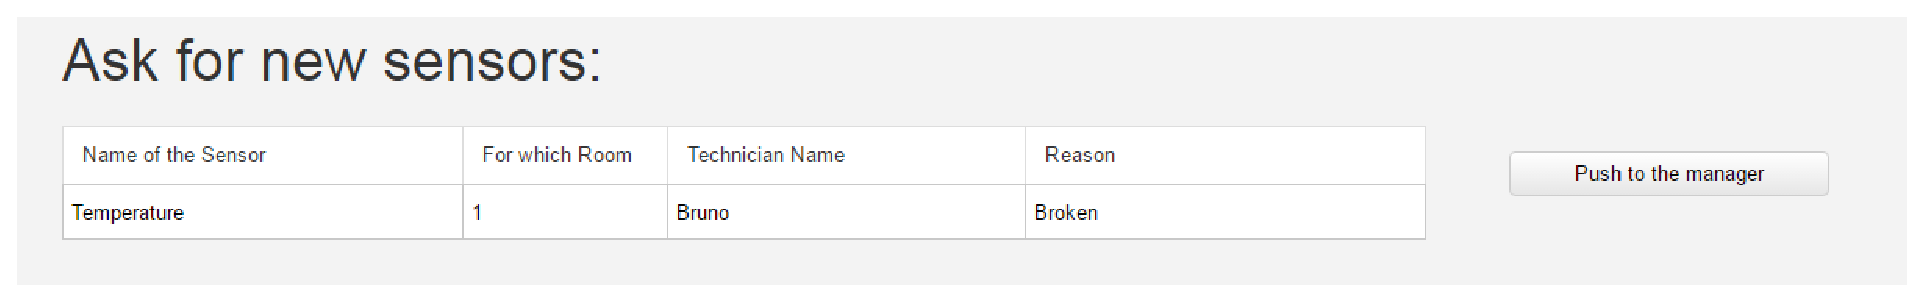
\includegraphics[width=1\textwidth]{images/AskForNewSensor.eps}
\end{figure} \\
2.\emph{RMS} displays a popup with the information entered by the Technician.\\
 \begin{figure}[h]
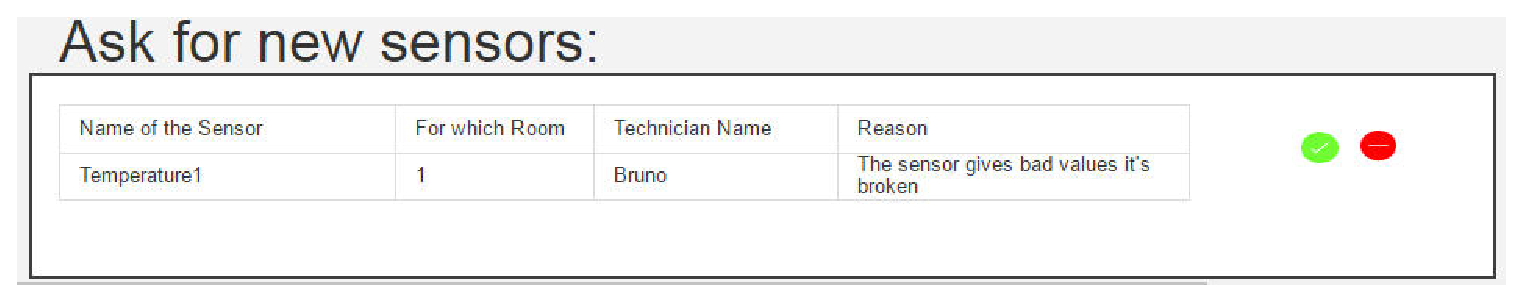
\includegraphics[width=1\textwidth]{images/AskForANewSensorPopUp.eps}
\end{figure}\\

3.\emph{Technician} accepts the information.\\

4.\emph{RMS} displays a message of validation and selects the values entered
from the \emph{Technician} and pushes them to the Manager request table.\\

5. \emph{Manager} accepts the request and instructs the \emph{RMS} to send a
confirmation to the Technician.\\

6. \emph{RMS} sets the value on the request sensor table from pending to true.\\
 \begin{figure}[h]
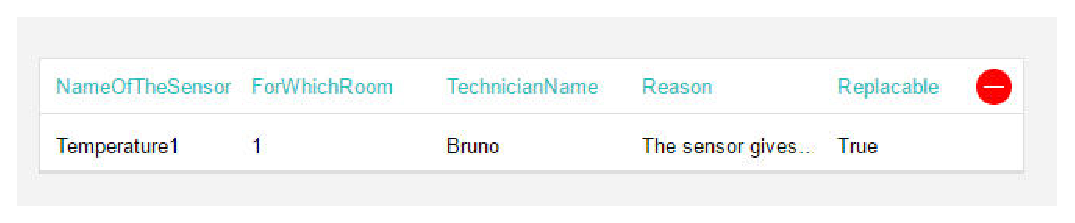
\includegraphics[width=1\textwidth]{images/AskForANewSensorTrue.eps}
\end{figure}\\

7. \emph{Technician} complets the fromular and presses add.\\
 \begin{figure}[h]
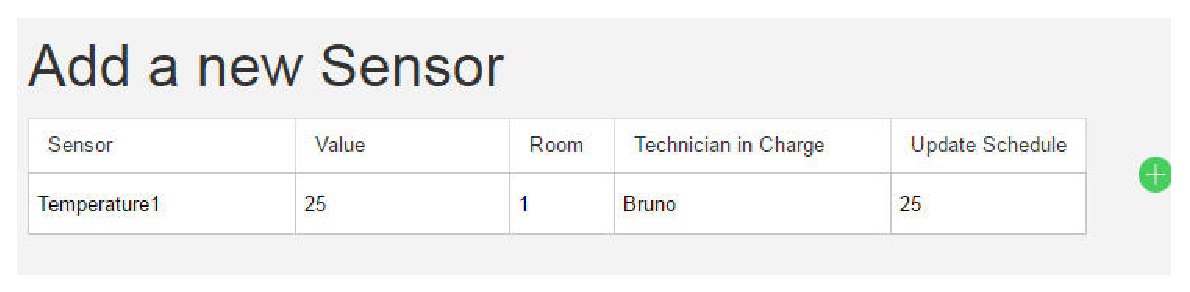
\includegraphics[width=1\textwidth]{images/AddANewSensorTechnician.eps}
\end{figure}\\

8. \emph{RMS} adds the sensor to the sensor table.\\

9.\emph{Technician} removes the sensor from the request sensor table by
pressing the red button.\\

 \begin{figure}[h]
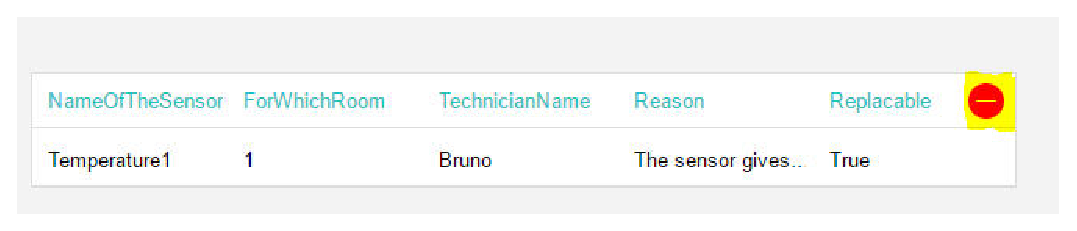
\includegraphics[width=1\textwidth]{images/RemoveSensorFromSensorRequestListTechnician.eps}
\end{figure}

10.\emph{RMS} displays a message of succesfully removed the sensor.\\
\item [\textbf{Extensions}]:\\
2.a Technician enters wrong input\\
\hspace*{0.5cm} 2.a.1 (5)-(8)\emph{EMS} displays the message error (5)-(8).
Action canceled.\\
\hspace*{0.5cm} \textbf{procedure restarts at step 1}\\
2.b Technician cancels action in the pop up.\\
\hspace*{0.5cm} \textbf{procedure restarts at step 1}\\
2.c Manager declines request\\
\hspace*{0.5cm} 2.b.1 \emph{RMS} informs \emph{Technician} that the request
has been declined.\\
}
\end{lyxlist}
\hrule
\vspace{0.5cm}

\break


\subsection{Request a different seed}
\vspace{0.5cm}
\hrule
\hfill
\begin{lyxlist}{PC1}
\small{
\item [\textbf{Procedure:}] Request a diffrent seed
\item [\textbf{Scope:}] Request Management System(\emph{RMS})
\item [\textbf{Primary Actor}:] Gardener
\item [\textbf{Secondary Actor(s)}:] Manager,\\
Error Management System
\item [\textbf{Goal:}] The intention that the Gardener can request a new
non already existing seed.
\item [\textbf{Level}:] User-goal level
\item [\textbf{Main~Success~Scenario}]:\\
1. \emph{Gardener} complets the input text fields and presses the ask new seed
button.\\
\item 
\begin{figure}[H]
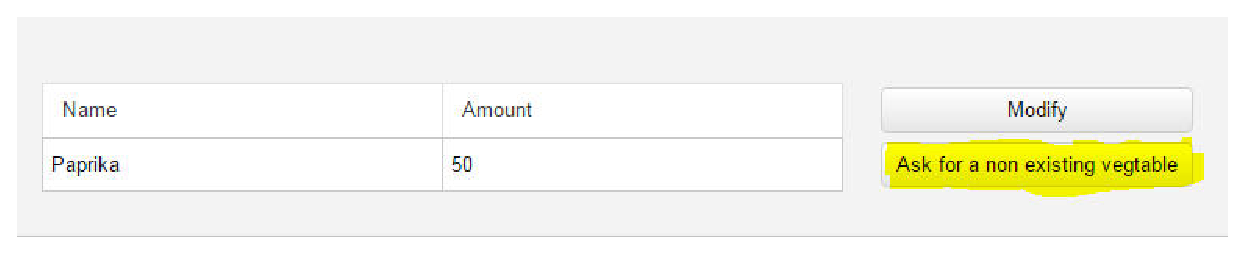
\includegraphics[width=1\textwidth]{images/AskForANonExistingVegtable.eps}
\end{figure}
2. \emph{RMS} displays a pop to show the input to the \emph{Gardener}\\
 \begin{figure}[H]
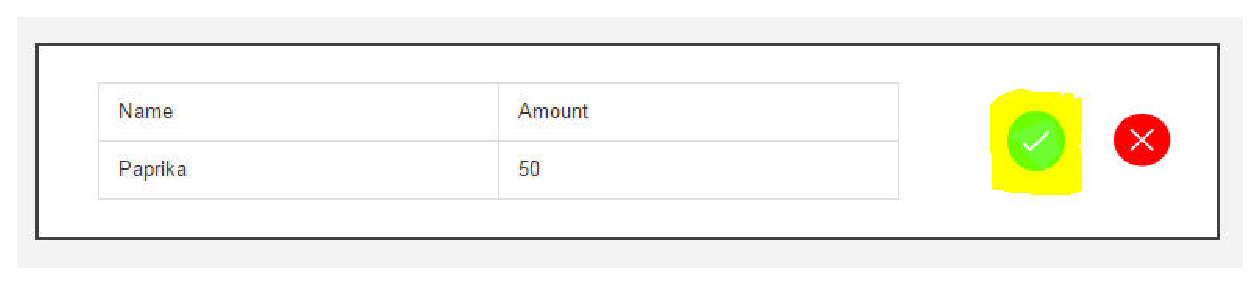
\includegraphics[width=1\textwidth]{images/AskForANonExistingVegtablePopUp.eps}
\end{figure}

3.\emph{Gardener} accepts the intput and instructs the \emph{RMS} to send
request.\\
4.\emph{RMS} pushes the input values to the manager request seed table.\\
5.\emph{Manager} accepts the request and instructs the \emph{RMS} to go on
the manager home screen.
 \begin{figure}[H]
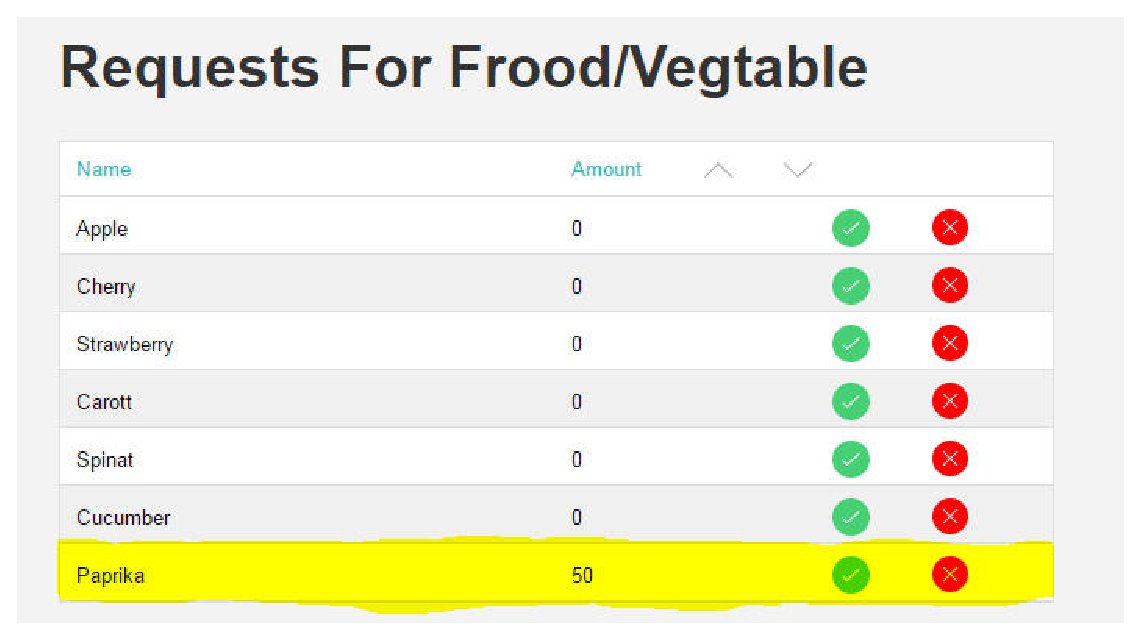
\includegraphics[width=1\textwidth]{images/AcceptRequestedCropManager.eps}
\end{figure}

6. \emph{Manager} complets the formula adding item to inventory and presses
add.\\
 \begin{figure}[H]
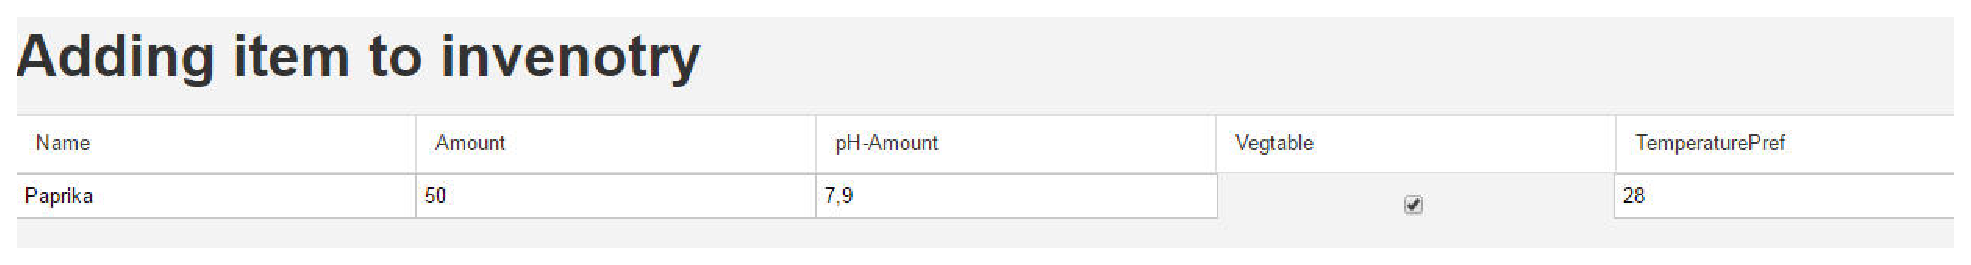
\includegraphics[width=1\textwidth]{images/AddingSeedToTheInventoryManager.eps}
\end{figure}

7. \emph{RMS} displays a pop up with the information written by the Manager.\\
8.\emph{Manager} validates the input and instructs the \emph{RMS} to update the
inventory.\\
 \begin{figure}[H]
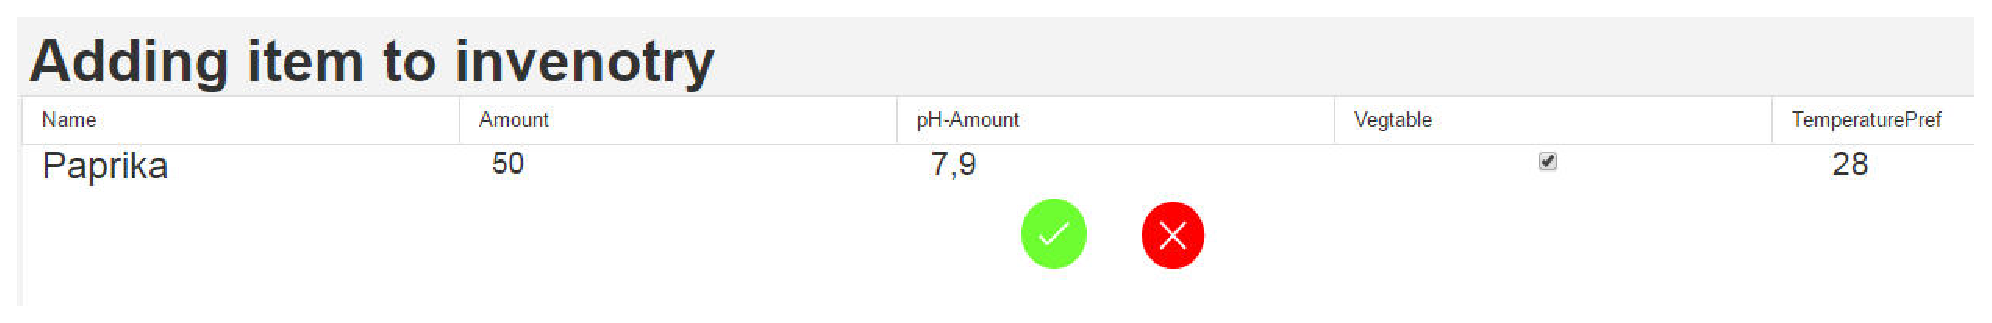
\includegraphics[width=1\textwidth]{images/AddingSeedToTheInventoryPopUp.eps}
\end{figure}

9. \emph{RMS} adds the given information to the crop invenotry table and
updates all the inventory tables.\\

\item [\textbf{Extensions}]:\\
2.a Gardener cancels the request\\
\hspace*{0.5cm} 2.a.1 {EMS} removes the pop up. Action canceled.\\
\hspace*{0.5cm} \textbf{procedure has stopped or can be resrarted at 1}
2.b Manager cancels the validation
\hspace*{0.5cm}2.b.1 {EMS} removes the pop up and cancels the action.\\
\hspace*{0.5cm}\textbf{procedure has stopped and can be restarted at 7.}
}
\end{lyxlist}
\hrule
\vspace{0.5cm}


\break
 
 
 
 

\subsection{Sign In}
\vspace{0.5cm}
\hrule
\hfill \break
\begin{lyxlist}{PC1}
\small{
\item [\textbf{Procedure:}] SignIn
\item [\textbf{Scope:}] Identified usage of the software
\item [\textbf{Primary Actor}:] User
\item [\textbf{Secondary Actor(s)}:] Greenhouse Software GS
\item [\textbf{Goal:}] Show the user GUI to manage the garden
\item [\textbf{Level}:] User-goal level
\item [\textbf{Main~Success~Scenario}]:\\
1. \emph{User} enters a username and password combination and signs in\\
2. \emph{GS} looks up the user rights defined by the administrator\\
3. \emph{GS} now show the correct Graphical User Interface (GUI) \emph{(Gardener, Technician, Manager or Administrator)} able to control the garden.
\item [\textbf{Extensions}]:\\
1.a Wrong username and password combination\\
\hspace*{0.5cm} 1.a.1 \emph{GS} notifies the \emph{User} that the entered information are wrong\\
\hspace*{0.5cm} \textbf{procedure recontinues at step 1}
}
\end{lyxlist}
\hrule
\vspace{0.5cm}


\break



\section{Mono-procedures}



\subsection{Technician}







\subsection{Manager}
\break




\subsection{Gardener}
\subsubsection{Retrive/Modify Crops from Table}

\vspace{0.5cm}
\hrule
\hfill \break
\begin{lyxlist}{PC1}
\small{
\item [\textbf{Procedure:}] Retrives vegtable or
frood the amount left of crops
\item [\textbf{Scope:}] Modify Management System \emph{MMS}
\item [\textbf{Primary Actor}:] Gardener,\\
Error Management System (EMS)
\item [\textbf{Goal:}] The intention that the gardner can retrive crops from
the inventory.
\item [\textbf{Level}:] User-goal level
\item [\textbf{Main~Success~Scenario}]:\\
1. \emph{Gardner} Complets the diffrent input text fields with there given
information and instructs the \emph{MMS} to retrive the crops by
pressing \emph{Modify}.\\

\begin{figure}
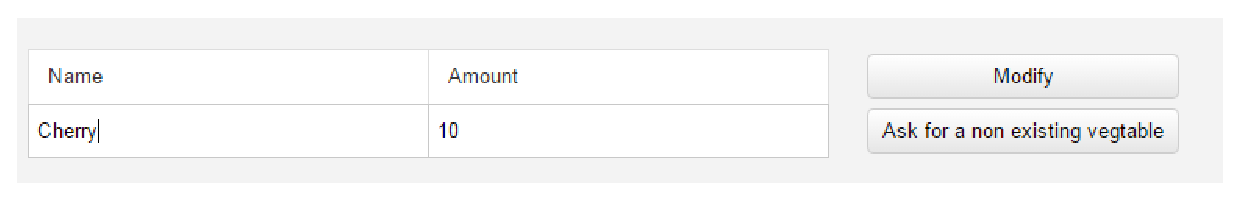
\includegraphics[width=1\textwidth]{images/RetriveCropsBase.eps}
\end{figure}

 2.{EMS} displays a pop up with the input entered by the \emph{Gardener}.\\
\begin{figure}
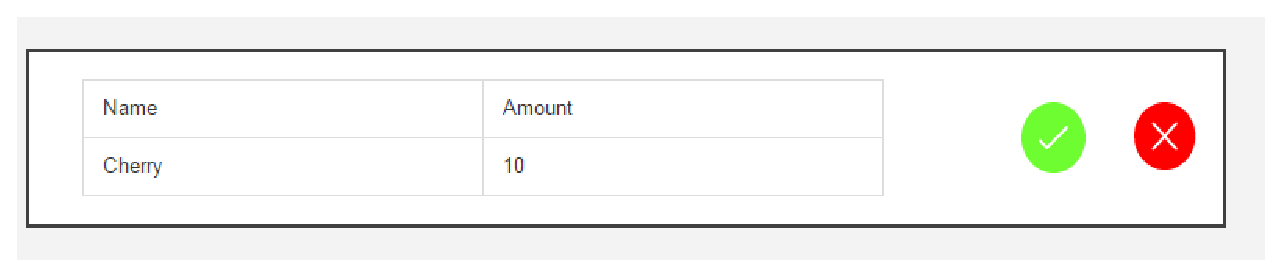
\includegraphics[width=1\textwidth]{images/PopUpRetrive.eps}
\end{figure}
3.\emph{Gardner} validates the input.\\
4.\emph{MMS} removes the crops from the table and updates the table.\\
5.\emph{MMS} enters new values to the Manager table at which time the crops
have been taken away.\\
\item [\textbf{Extensions}]:\\
2.a  \emph{Gardener} declines the pop up request to retrive crops.\\
\hspace*{0.5cm} 2.a.1 \emph{EMS}  disables the pop up and action has been
canceld\\
\hspace*{0.5cm} \textbf{procedure continues at step 1 or can be anulated}
\item 
}
\end{lyxlist}
\hrule
\vspace{0.5cm}


\break
\subsubsection{MyProcedure2MyActor2}
\ldots















\newpage

% Software operations
\chapter{Software operations}
\label{chap:soptware_operations}


Explain each allowed software operations (i.e. an atomic unit of treatment, a service, a functionality) including a brief description of the operation, required parameters, optional parameters, default options, required steps to trigger the operation, assumptions upon request of the operation and expected results of executing such operation.
Describe how to recognise that the operation has successfully been executed or
abnormally terminated. The template given below (i.e. section \ref{operation:MyOperation} has to be used).

Group the operations devoted to the needs of specific actors. Common
operations to several actors may be grouped and presented once to avoid redundancy.


\section{Adding task to gardeners schedule}

\hrule
\hfill
\vspace{0.5cm}
\label{operation:addTaskGardener}

The manager creates and adds a new task to be added to gardener's schedule.
\begin{description}

\item \textbf{Parameters:} nameTask, taskDescription, room, nameGardener, date,
importance
\item \textbf{Precondition:} The manager is logged in and on the manage gardener
schedule screen
\item \textbf{Post-condition:} A new task has been added to the schedule and the
new task has been assigned to the specified gardener and the manager is
notified that the task has been added.
\item \textbf{Output messages:} The \textbf{manager} will be notified that the
task has been created.

\item \textbf{Triggering:}
\begin{enumerate}
\item From within the manage gardener schedule screen, the \textbf{manger} fills
out the required entries related to the task information like the name of the task or
the date and clicks on the add button.
\item The system then adds the task now to the schedule of the gardener.
\end{enumerate}
\end{description}
\subsection{Example of adding a task}
The \textbf{manager} wants to add a watering task to the schedule, so fills out
the textinputfields as shown in the image and then he clicks on the add button.
 \begin{figure}
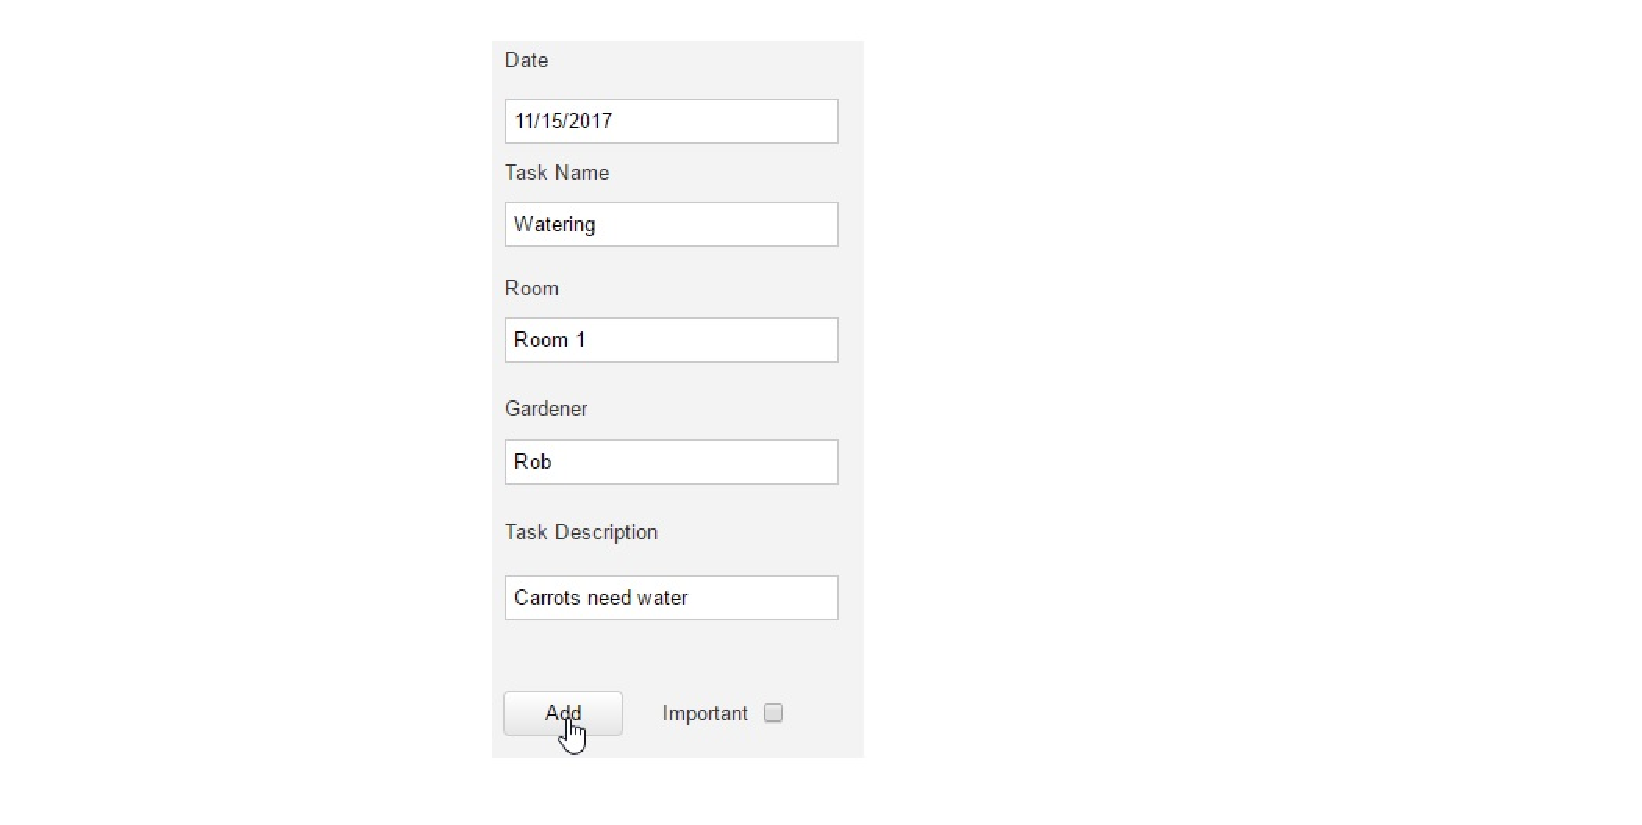
\includegraphics[width=1\textwidth]{images/addingTaskGardener.eps}
 \end{figure}


\section{Adding task to technician schedule}

\hrule
\hfill
\vspace{0.5cm}
\label{operation:addTaskTechnichian}

The manager creates and adds a new task to be added to technician's schedule.
\begin{description}

\item \textbf{Parameters:} nameTask, taskDescription, room, nameTechnician,
date, importance
\item \textbf{Precondition:} The manager is logged in and on the manage gardener
schedule screen.
\item \textbf{Post-condition:} A new task has been added to the schedule and the
new task has been assigned to the specified technician and the manager is
notified that the task has been added.
\item \textbf{Output messages:} The \textbf{manager} will be notified that the
task has been created.

\item \textbf{Triggering:}
\begin{enumerate}
\item From within the managa technician schedule screen, the \textbf{manger}
fills out the required entries related to the task information like the name of the task or
the date and clicks on the add button.
\item The \textbf{manager} The system now adds the task to the schedule of the
technician.
\end{enumerate}
\end{description}
\subsection{Example of adding a task}
The \textbf{manager} wants to the technician to change sensors, so he fills out
the requied fields and then presses the add button as shown in the image.



\section{Request a new sensor}

\hrule
\hfill
\vspace{0.5cm}
\label{operation:Request a new sensor}

The Technician can request a new sensor.
\begin{description}
\item \textbf{Parameters:} NameSensor,RoomNumber,TechnicianName,Reason
\item \textbf{Precondition:} The system is bootedup and the technician has to be
logged in and be on the technician screen.
\item \textbf{Post-condition:} Updated request sensor table.
\item \textbf{Output messages:}Message with the request pulled to the manager.
\item \textbf{Triggering:}
\begin{enumerate}
\item \textbf{Technician} Complets the diffrent input fields and presses the
button push to the manager.
\begin{figure}[H]
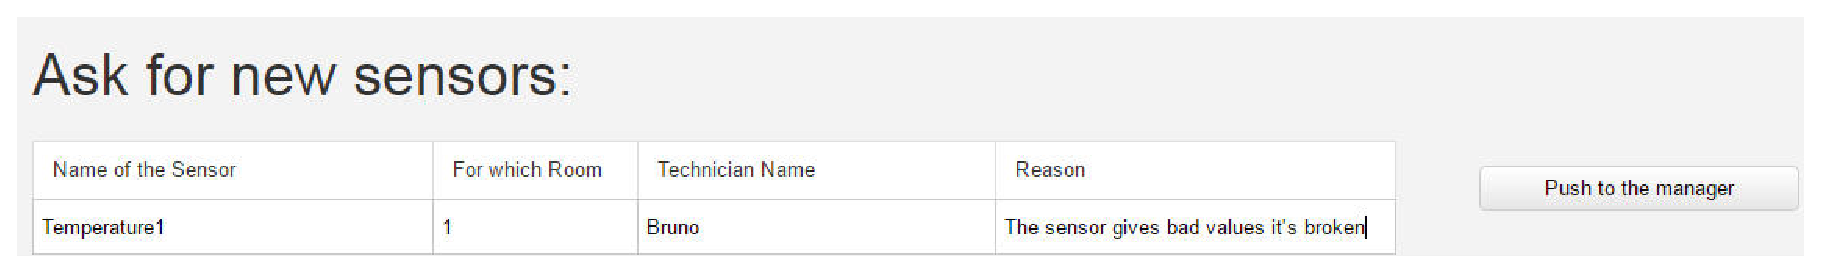
\includegraphics[width=1\textwidth]{images/AskForANewSensor.eps}
\end{figure}
\item System sends the information to the manager by updating the request
sensor table.
\end{enumerate}
\end{description}

\subsection{Example of a request of a sensor}
\textbf{Technician} complets the input text field with their given information
that means Name of the Sensor:Temperature1 RoomNumber:1 Technician Name: Bruno
and Reason Sensor Temperature 1 gives wrong information sensor is
damaged.\textbf{System} inserts this information to the manager request sensor
table.
\hfill
\vspace{0.5cm}
\hrule

\section{Accept the request for a new sensor}

\hrule
\hfill
\vspace{0.5cm}

\label{operation:Accept the request for a new sensor}

The Manager can accept a new sensor.
\begin{description}
\item \textbf{Parameters:} /
\item \textbf{Precondition:} The system is bootedup and the Manager has to be
logged in and be on the Manager request screen and a request has to be
available.
\item \textbf{Post-condition:} Validation of the request send to the Technician.
\item \textbf{Output messages:}Successfully allowed to replace the sensor.
\item \textbf{Triggering:}
\begin{enumerate}
\item \textbf{Manager} Presses the green button to validate the request.
\item System sends a message that the sensor can be added to the room to the
technican.
\item \begin{figure}[H]
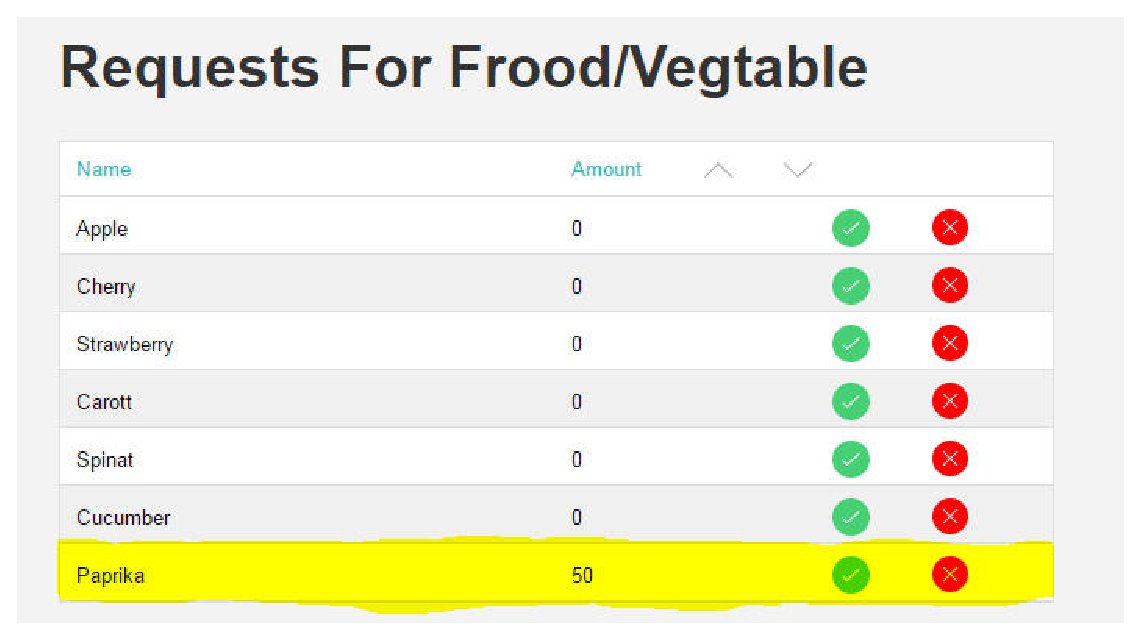
\includegraphics[width=1\textwidth]{images/AcceptRequestedCropManager.eps}
\end{figure}
\end{enumerate}
\end{description}

\subsection{Example of accepting a request}
\textbf{Maneger} presses the green button to accept the request from the
Temperature1 Sensor. \textbf{System} sends a validation message to the gardener.
\hfill
\vspace{0.5cm}
\hrule

\break

\section{Add a new sensor}

\hrule
\hfill
\vspace{0.5cm}

\label{operation:Add a new sensor}
The Technician can add a sensor which has been maid available from the manager.
\begin{description}
\item \textbf{Parameters:} SensorName,Value,Room,TechnicianName,UpdateSchedule
\item \textbf{Precondition:} The system is bootedup and the Technician has to be
logged in and be on the Tehcnician screen and a request to add a sensor has to
be available.
\item \textbf{Post-condition:} The sensor has been successfully updated with the
sensor which has been added.
\item \textbf{Output messages:}Successfully added the sensor to the Sensor List.
\item \textbf{Triggering:}
\begin{enumerate}
\item \textbf{Technician} complets the diffrent input text fields and presses
the green add button .
\begin{figure}[H]
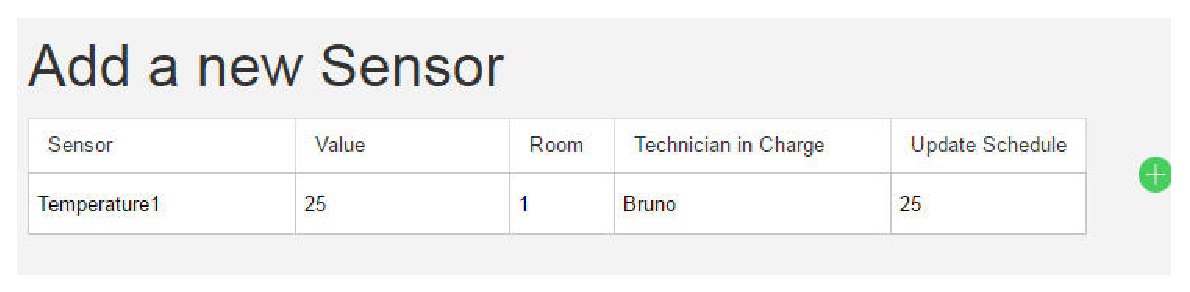
\includegraphics[width=1\textwidth]{images/AddANewSensorTechnician.eps}
\end{figure}
\item System pushes now the information to the sensor table and updates it by
adding the sensor with the other informations added.
\end{enumerate}
\end{description}

\subsection{Example of adding a new sensor}
\textbf{Technician} complets the given input text fields with the sensor name
:Temperature1 value 32 degrees and the room: 1 technician name :Bruno and the
update schedule is 15. \textbf{System} pushes the information to the sensor
table and displays the new updated table.
\hfill
\vspace{0.5cm}
\hrule



\section{Remove  requested sensor}

\hrule
\hfill
\vspace{0.5cm}
\label{operation:Remove a new sensor}

The Technician can remove the requested sensor from the request table.
\begin{description}
\item \textbf{Parameters:} /
\item \textbf{Precondition:} The system is bootedup and the technician has to be
logged in and be on the technician screen and a request should be in the
request sensor table.
\item \textbf{Post-condition:} Removes the requested sensor from the sensor
request table.
\item \textbf{Output messages:} Successfully deleted the requested sensor.
\item \textbf{Triggering:}
\begin{enumerate}
\item \textbf{Technician} presses the red button on request sensor table.
\begin{figure}[H]
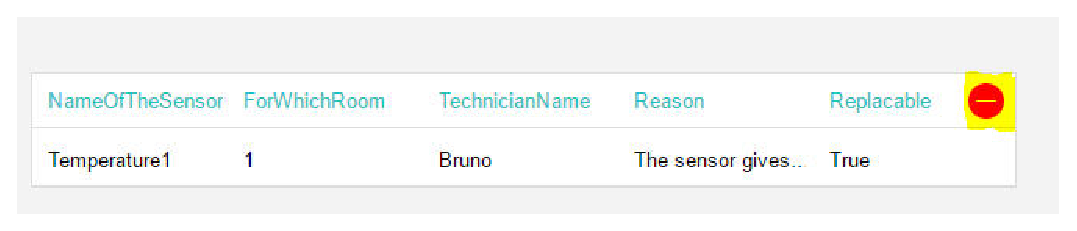
\includegraphics[width=1\textwidth]{images/RemoveSensorFromSensorRequestListTechnician.eps}
\end{figure}
\item System removes sensor from the request table.
\end{enumerate}
\end{description}

\subsection{Example of a removing of a sensor}
\textbf{Technician} presses the red button on the ligne 1 of the table where
temperature1 and which room = 1. The system removes the sensor from the request
list.

\hfill
\vspace{0.5cm}
\hrule



\break



\section{Ask for a diffrent seed}

\hrule
\hfill
\vspace{0.5cm}

\label{operation:Ask for a diffrent seed}

The gardener can request a diffrent seed which isn't already in the crops
inventory.
\begin{description}
\item \textbf{Parameters:} SeedName,Amount
\item \textbf{Precondition:} The system is bootedup and the Gardener has to be
logged in and be on the Gardener screen.
\item \textbf{Post-condition:} The request has been send by adding it on the
request seed table.
\item \item \textbf{Output messages:}Reqeust has been send.
\item \textbf{Triggering:}
\begin{enumerate}
\item \textbf{Gardener} complets the diffrent input text fields and presses
the ask for a non existing seed button.
\begin{figure}[H]
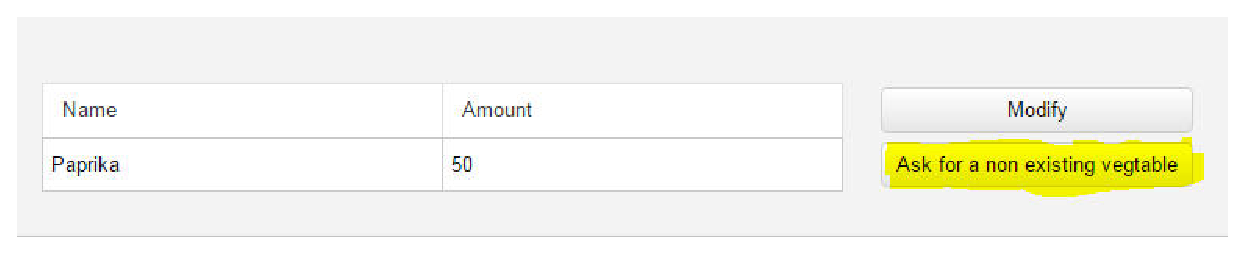
\includegraphics[width=1\textwidth]{images/AskForANonExistingVegtable.eps}
\end{figure}
\item \textbf{System} displays a pop up of the entered information.
\begin{figure}[H]
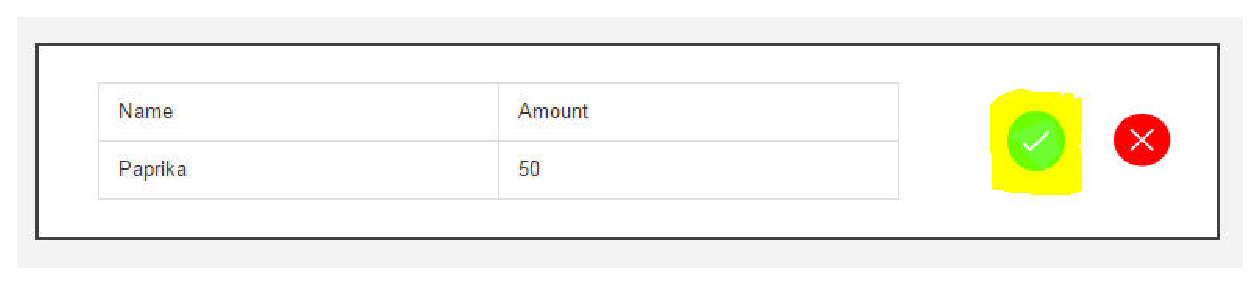
\includegraphics[width=1\textwidth]{images/AskForANonExistingVegtablePopUp.eps}
\end{figure}
\item \textbf{Gardener} accepts the pop up.
\item \textbf{System} pushes the information to the manager request seed table
and updates it.
\end{enumerate}
\end{description}

\subsection{Example of accepting a request}
\textbf{Technician} complets the given input text fields with the Name Mango and
amount 50. \textbf{System} displays the pop up of the information enterer Mango
and 50.\textbf{Gardener} accepts the pop up.\textbf{System} updates the request
crop table by adding Mango and amount to the table.
\hfill
\vspace{0.5cm}
\hrule


\section{Accept a diffrent seed}

\hrule
\hfill
\vspace{0.5cm}

\label{operation:Accept a diffrent seed}

The Manager can accept the request for a new seed which is not already on the
crop inventory table.
\begin{description}
\item \textbf{Parameters:}seedName
\item \textbf{Precondition:} The system is bootedup and the Manager has to be
logged in and be on the Manager request screen.
\item \textbf{Post-condition:} The request has been validated manager
redirected to the manager home screen.
\item \item \textbf{Output messages:} Successfully accepted now add a the seed
to the storage/inventory.
\item \textbf{Triggering:}
\begin{enumerate}
\item \textbf{Manager} presses the green button to validated the request.
\item \textbf{System}redirects the manager to the manager home screen and
displays the output message.

\end{enumerate}
\end{description}

\subsection{Example of accepting a request}
\textbf{Manager} accepts by pressing the green button on COCO with the amount
50.\textbf{System} displays a successfully accepted and redirects the manager
to the ma,ager homescreen.
\textbf{Manager}complets the di\ldots\ldots.;;
\hfill
\vspace{0.5cm}
\hrule
 
\break


\section{Remove Seed from Inventory}

\hrule
\hfill
\vspace{0.5cm}

\label{operation:RemoveSeed}

The manager can remove a given kind of seed completly.
\begin{description}

\item \textbf{Parameters:} NameSeed, Amount
\item \textbf{Precondition:} The system is bootedup and manager has to be
logged in and be on the manager request screen.
\item \textbf{Post-condition:} Request table has been updated with the removed
seed.
\item \textbf{Output messages:} Successfully removed item.
\item \textbf{Triggering:}
\begin{enumerate}
\item \textbf{Manager} presses the red button on the crops inventory table.
\item \begin{figure}[H]
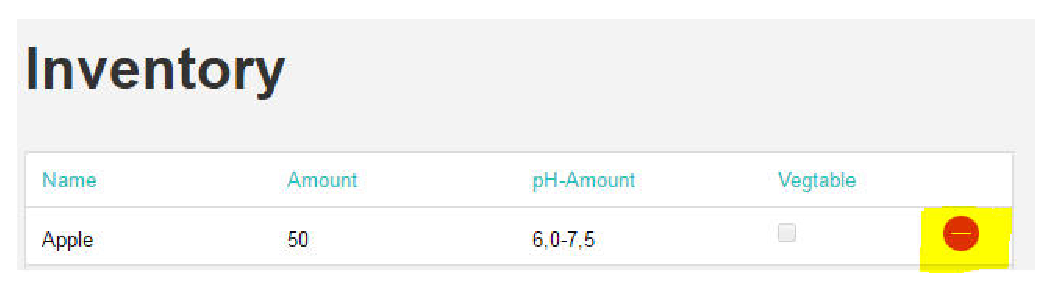
\includegraphics[width=1\textwidth]{images/RemoveSeedFromInventory.eps}
\end{figure}
\item System removes the crops from the crops inventory on the manager and
gardener screen.
\end{enumerate}
\end{description}

\subsection{Example of removing crops}
\textbf{Manager} removes the crops by pressing the red button. The System
updates the changes on the manager request screen and Gardener screen.
\hfill
\vspace{0.5cm}
\hrule


\section{Sort request crops by amount ascending order}

\hrule
\hfill
\vspace{0.5cm}

\label{operation:sortSeedRequest}

The manager can sort the crops which are requested by ascanding order.
\begin{description}

\item \textbf{Parameters:} /
\item \textbf{Precondition:} The system is bootedup and manager has to be
logged in and be on the manager request screen.
\item \textbf{Post-condition:} Request seed table has been ordered in ascanding
order.

\item \textbf{Output messages:} none
\item \textbf{Triggering:}
\begin{enumerate}
\item \textbf{Manager} presses the top arrow.
\item System sorts the list by amount value by ascending order.
\begin{figure}[H]
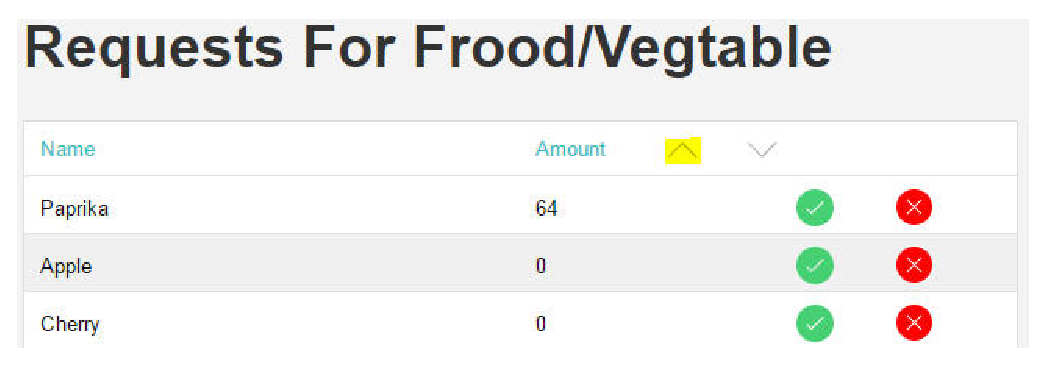
\includegraphics[width=1\textwidth]{images/RequestByAscendingOrderManager.eps}
\end{figure}
\end{enumerate}
\end{description}

\subsection{Example of removing crops}
\textbf{Manager} presses the arraw on the request crop table. System sorts the
the table by amount in ascending order.

\hfill
\vspace{0.5cm}
\hrule

\break

\section{Modify/Retrive seed Amount}

\hrule
\hfill
\vspace{0.5cm}
\label{operation:modifySeedAmount}


The \textbf{Gardener} can modify the amount of seed on the crops inventory
table.
\begin{description}
\item \textbf{Parameters:} Name,amount
\item \textbf{Precondition:} The system is bootedup and the gardener has to be
logged in and be on the Gardener sreen.
\item \textbf{Post-condition:} Seed inventory has been modifyed on manager and
gardener screen.
\item \textbf{Output messages:} Successfully retrived seeds from inventory
\item \textbf{Triggering:}
\begin{enumerate}
\item \textbf{Gardener} Complets the input text fields and presses the modify
button.
\begin{figure}[H]
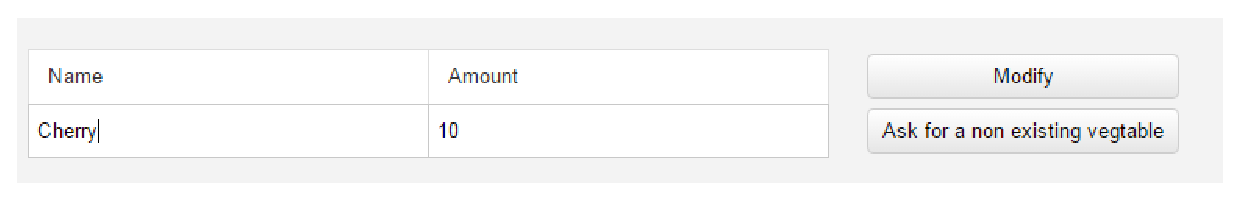
\includegraphics[width=1\textwidth]{images/RetriveCropsBase.eps}
\end{figure}
\item System updates the table of crop inventory and adds a the time of
retriving to the manager retriving Gardener table adn reloads the screen.
\end{enumerate}
\end{description}

\subsection{Example of removing crops}
\textbf{Gardener} enters the two input fields name = Tomatoe and amount=10.
The system retrives the amount which is equal to 10 from the inventory amount of
the name Tomatoe.
\hfill
\vspace{0.5cm}
\hrule





\section{Add seed to the inventory request Gardener}

\hrule
\hfill
\vspace{0.5cm}

\label{operation:Add a diffrent seed request Gardener}

The Manager can add a new seed to the inventory.
\begin{description}
\item
\textbf{Parameters:}Name,Amount,ph-Amount,Vegtable(boolean),TemperaturePreference
\item \textbf{Precondition:} The system is bootedup and the Manager has to be
logged in and be on the Manager screen and a request has to be accepted by the
manager.
\item \textbf{Post-condition:} The invenotry has been updated by adding the
attributes to the table.
\item 
\item \item \textbf{Output messages:} Successfully accepted the request
\item \textbf{Triggering:}
\begin{enumerate}
\item \textbf{Manager} complets the formula and presses the add button.
\begin{figure}[H]
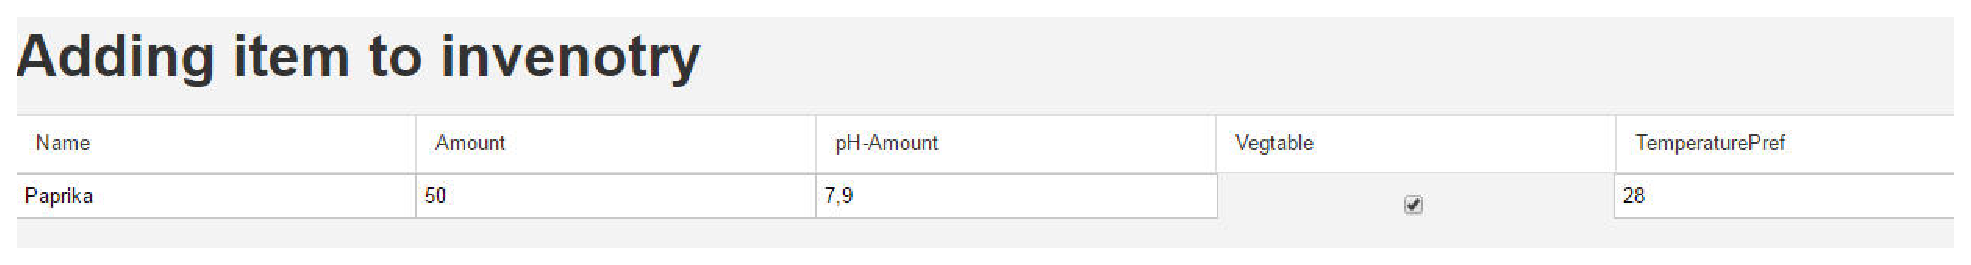
\includegraphics[width=1\textwidth]{images/AddingSeedToTheInventoryManager.eps}
\end{figure}
\item \textbf{System} shows a pop up of the entered values.
\begin{figure}[H]
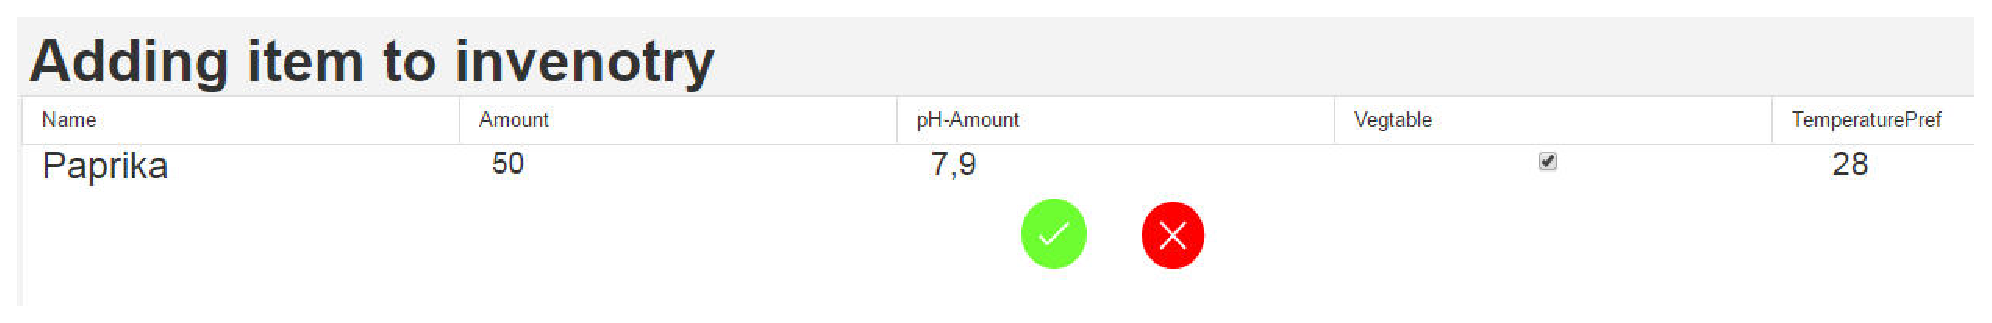
\includegraphics[width=1\textwidth]{images/AddingSeedToTheInventoryPopUp.eps}
\end{figure}
\item \textbf{Manager} accepts the pop up request.
\item \textbf{System} displays a message of success and adds the values to the
inventory crop table.

\end{enumerate}
\end{description}

\subsection{Example of accepting a request}
\textbf{Manager} complets the given inputs text field with the
Name: Coconut and amount 50 and ph value 9 and Vegtable false
(not coching the crop field) and temperature preference : 34. \textbf{System}
displays a pop up  what the user has entered in this case Coconut 50 9 (false)
and 34.Manager accepts the pop up by pressing the green button. System updates
the crop inventory table by adding the input values from the manager to the
table.
\hfill
\vspace{0.5cm}
\hrule












\break

\section{Filter by sensor type}

\hrule
\hfill
\vspace{0.5cm}

\label{operation:filterSensorTable}

The \textbf{Technician} can filter the table by filter type.
\begin{description}

\item \textbf{Parameters:} /
\item \textbf{Precondition:} The system is bootedup and Technician has to be
logged in and be on the technician screen.
\item \textbf{Post-condition:} The table on the screens show only the filtered
values.
\item \textbf{Output messages:} none
\item \textbf{Triggering:}
\begin{enumerate}
\item \textbf{Technician} choses on the top down menu a sensor type.
\begin{figure}[H]
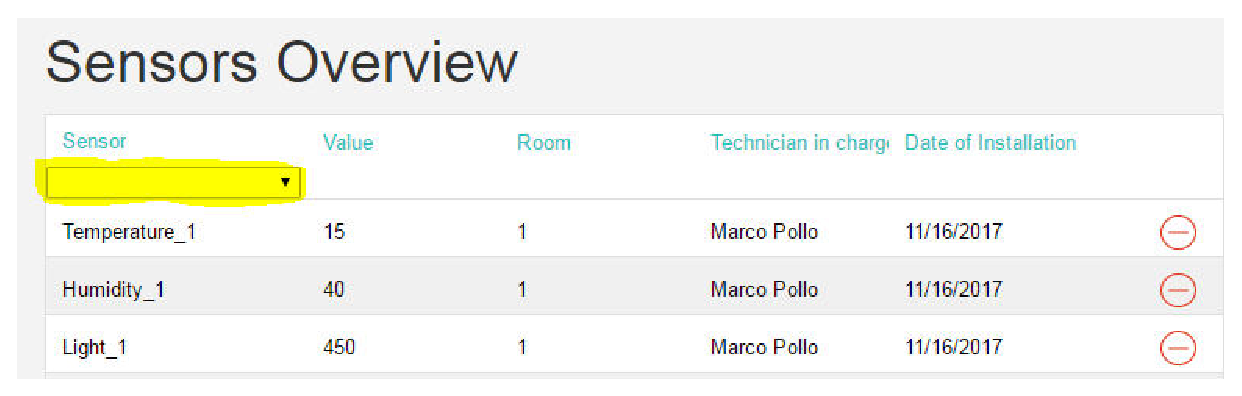
\includegraphics[width=1\textwidth]{images/FilterSensorByTypeTechnician.eps}
\end{figure}
\item System filters out all the non equal types and doesn't display them.
\end{enumerate}
\end{description}

\subsection{Example of filtering the Sensors}
\textbf{Technician} choses a type on a the top down menu Temperature. System
know doesn't display the sensor where the type isn't equal to Temperature.
\hfill
\vspace{0.5cm}
\hrule






\section{Removes sensor from Sensor Array}

\hrule
\hfill
\vspace{0.5cm}

\label{operation:removesSensor}

The \textbf{Technician} removes the a specific sensor from the table.
\begin{description}

\item \textbf{Parameters:} /
\item \textbf{Precondition:} The system is bootedup and Technician has to be
logged in and be on the technician screen.
\item \textbf{Post-condition:} The table of sensors has been updated on the
technician and gardener screen.
\item \textbf{Output messages:} none
\item \textbf{Triggering:}
\begin{enumerate}
\item \textbf{Technician} choses the sensor which he wants to delete and presses
the red button.
\begin{figure}[H]
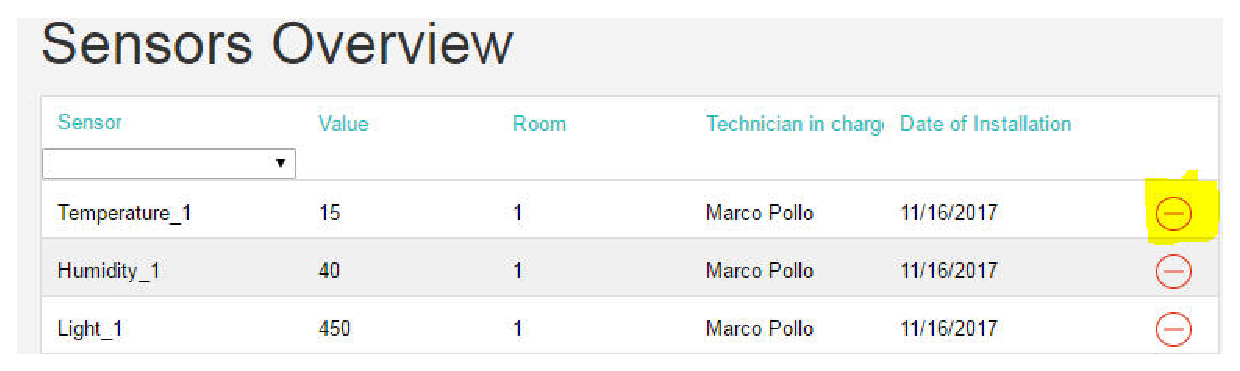
\includegraphics[width=1\textwidth]{images/RemoveSensorFromSensorListTechnician.eps}
\end{figure}
\item System removes the sensor from the table.
\end{enumerate}
\end{description}

\subsection{Example of removing Sensor}
\textbf{Technician} choses a given sensors on the Sensor table Temperature 1
sensor and presses the red button on the same line.
System removes the line from the table and reloads the screen to update it.

 \hfill
\vspace{0.5cm}
\hrule



\break
\section{Build Temperature Line Diagram}
\label{operation:BuildTemperatureDiagram}
The system draws the line diagram for the temperature of the selected room of
the dropdown menu next to it.

\begin{description}

\item \textbf{Parameters:} HistoryOfTemperaturesInAllRooms
\item \textbf{Precondition:} The system is bootedup and any actor is logged in.
\item \textbf{Post-condition:} The corresponding diagram will be drawn and
shown.

\item \textbf{Triggering:}
\begin{enumerate}
\item If at any time the \emph{statistics} page is accessed.
\end{enumerate}
\end{description}

\subsection{Example of Build Temperature Line Diagram}
The logged in user wants to see the statistics of the past days.
The user clicks on the \emph{statistics} page in the menu.
The system will now draw the temperature line diagram.




\section{Build Current Stock Bar Diagram}
\label{operation:BuildCurrentStockDiagram}
The system draws the bar diagram of the current stock of the inventory.

\begin{description}

\item \textbf{Parameters:} CurrentStockOfSeeds
\item \textbf{Precondition:} The system is bootedup and any actor is logged in.
\item \textbf{Post-condition:} The corresponding diagram will be drawn and
shown.

\item \textbf{Triggering:}
\begin{enumerate}
\item If at any time the \emph{statistics} page is accessed.
\end{enumerate}
\end{description}

\subsection{Example of Build Current Stock Bar Diagram}
The logged in user wants to see the current stock of the inventory.
The user clicks on the \emph{statistics} page in the menu.
The system will now draw the current stock bar diagram.



\break
\section{Build Water Consumption And Luminosity Level Bar And Line Diagram}
\label{operation:BuildWaterConsumptionAndLuminosityLevelDiagram}
The system draws the bar and line diagram for the water consumption in
milliliter and the luminosity level in spectral power of the selected room of
the dropdown menu next to it.

\begin{description}

\item \textbf{Parameters:} HistoryOfWaterConsumptionInAllRooms,
HistoryOfLuminosityLevelInAllRooms
\item \textbf{Precondition:} The system is bootedup and any actor is logged in.
\item \textbf{Post-condition:} The corresponding diagram will be drawn and
shown.

\item \textbf{Triggering:}
\begin{enumerate}
\item If at any time the \emph{statistics} page is accessed.
\end{enumerate}
\end{description}

\subsection{Example of Build Water Consumption And Luminosity Level Bar And Line
Diagram}
The logged in user wants to see the statistics of the past days.
The user clicks on the \emph{statistics} page in the menu.
The system will now draw the temperature line diagram.




\section{Show Crop statistics}
\label{operation:ShowCropStatistics}
The system shows the statistics of the crop \emph{(Date harvested, Plant
harvested, Number of plants harvested, Total weigth of the harvest)} and
calulates the \emph{Average weigth/plant, Days until the plants were harvested
and the growth per day}.

\begin{description}

\item \textbf{Parameters:} DatePlanted, DateHarvested, PlantHarvested,
NumberOfPlants, TotalWeigthOfCrop
\item \textbf{Precondition:} The system is bootedup and any actor is logged in.
\item \textbf{Post-condition:} The corresponding information will be calculated
and shown.

\item \textbf{Triggering:}
\begin{enumerate}
\item If at any time the \emph{statistics} page is accessed.
\item The logged in user chooses a different crop from the crop list on the
\emph{statistics} page.
\end{enumerate}
\end{description}


\subsection{Example of Show Crop statistics}
The logged in user wants to see the statistics of the past crops.
The user clicks on the \emph{statistics} page in the menu.
The system will now calculate and show the information on the latest crop.
The user wants to see older crops and triggers this system operation by choosing
a different crop.


\break
\section{Automatical Creation of Alert for Sensors}
\label{operation:AddAlertForSensors}
The system checks the incoming signal from all the different sensors for invalid
data or no incoming signal.

\begin{description}

\item \textbf{Parameters:} SensorData
\item \textbf{Precondition:} The system is bootedup.
\item \textbf{Post-condition:} AlertsDatabase is updated with a new entry.

\item \textbf{Triggering:}
\begin{enumerate}
\item The Sensors transmit invalid or impossible data.
\item The Sensors transmit no data.
\end{enumerate}
\end{description}

\subsection{Example of Automatical Creation of Alert for Sensors}
The system is bootedup and is monitoring the signal of the sensors.
Now one of the sensors sends invalid data (example: Humidity Sensor sends data
with more than 100 percent humidity) or lost the connection for whatever reason
to the system, an entry will be added into the alerts database.




\section{Automatical Creation of Alert for Warnings}
\label{operation:AddAlertForWarnigns}
The system checks the incoming signal from the humidity and temperature sensors
for data which is out of the pre-defined range.

\begin{description}

\item \textbf{Parameters:} SensorData
\item \textbf{Precondition:} The system is bootedup.
\item \textbf{Post-condition:} AlertsDatabase is updated with a new entry.

\item \textbf{Triggering:}
\begin{enumerate}
\item The Sensors transmit data out of the pre-defined range
\end{enumerate}
\end{description}

\subsection{Example of Automatical Creation of Alert for Warnings}
The system is bootedup and is monitoring the signal of the sensors.
Now the temperature sensors sends a temperature of 18 degrees celsius. The
pre-defined range for the temperature is from 20 to 27 degrees. The system will
add a warning to the alerts database, the temperature is too low.






\break



\section{Humidty sensor push information}

\hrule
\hfill
\vspace{0.5cm}
\label{operation:Humidty sensor push information}

The Humidity Sensor pushes the information to the sensor table.
\begin{description}
\item \textbf{Parameters:} 
\item \textbf{Precondition:} The system is bootedup with the respected
configurations.
\item \textbf{Post-condition:} Updated sensor value in sensor table.

\item \textbf{Triggering:}
\begin{enumerate}
\item \textbf{Humidity sensor} send digital signal to the system.
\item System updates the value of the given sensor in the sensor table.
\begin{figure}[H]
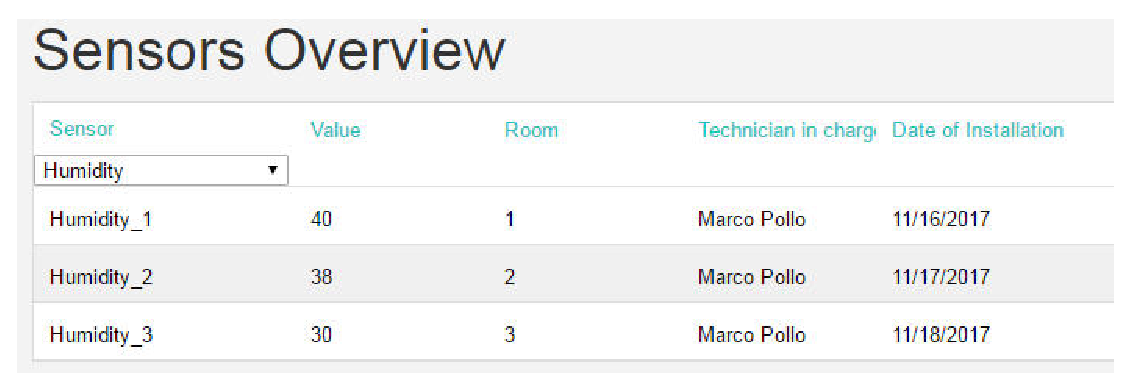
\includegraphics[width=1\textwidth]{images/HumiditySensor.eps}
\end{figure}
\end{enumerate}
\end{description}

\subsection{Example of humidity sensor sending digital signal}
\textbf{Humidity sensor 1} sends 40 as digital signal. \textbf{System} updates
the sensor table value from room 1 and humidity sensor1.
\hfill
\vspace{0.5cm}
\hrule


\section{Temperature sensor push information}

\hrule
\hfill
\vspace{0.5cm}
\label{operation:Temperature sensor push information}

The Temperature Sensor pushes the information to the sensor table.
\begin{description}
\item \textbf{Parameters:} 
\item \textbf{Precondition:} The system is bootedup with the respected
configurations.
\item \textbf{Post-condition:} Updated sensor value in sensor table.

\item \textbf{Triggering:}
\begin{enumerate}
\item \textbf{Temperature sensor} sends digital signal to the system.
\item System updates the value of the given temperature sensor in the sensor
table.
\item \begin{figure}[H]
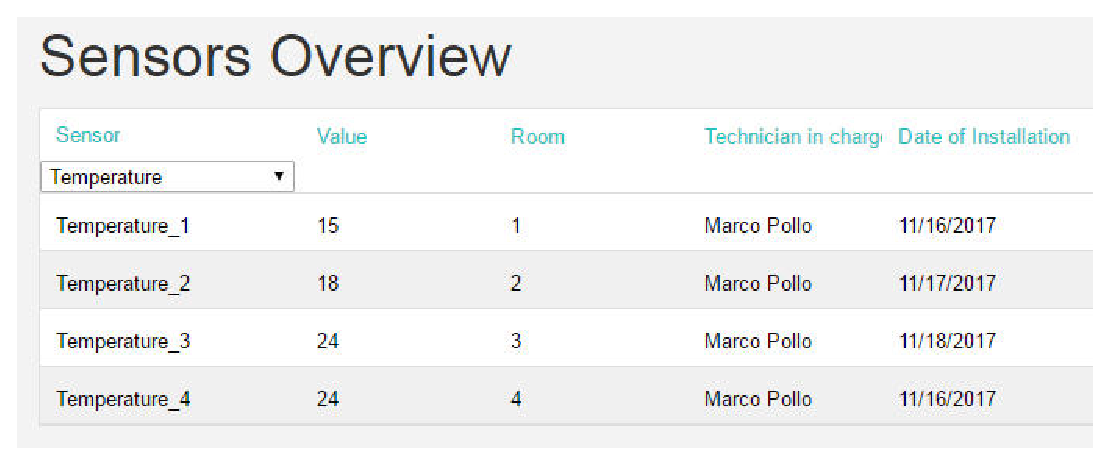
\includegraphics[width=1\textwidth]{images/TemperatureSensor.eps}
\end{figure}
\end{enumerate}
\end{description}

\subsection{Example of humidity sensor sending digital signal}
\textbf{Temperature sensor 1} sends 24 as digital signal. \textbf{System}
updates the sensor table value from room 1 and Temperature sensor1 by modifing
the value to 24.
\hfill
\vspace{0.5cm}
\hrule

\break
\section{Light sensor push information}

\hrule
\hfill
\vspace{0.5cm}
\label{operation:Light sensor push information}

The  Light Sensor pushes the information to the sensor table.
\begin{description}
\item \textbf{Parameters:} 
\item \textbf{Precondition:} The system is bootedup with the respected
configurations.
\item \textbf{Post-condition:} Updated Light value in sensor table of the given
Light sensor.

\item \textbf{Triggering:}
\begin{enumerate}
\item \textbf{Light sensor} sends digital signal to the system.
\item System updates the value of the given sensor in the sensor table.
\item \begin{figure}[H]
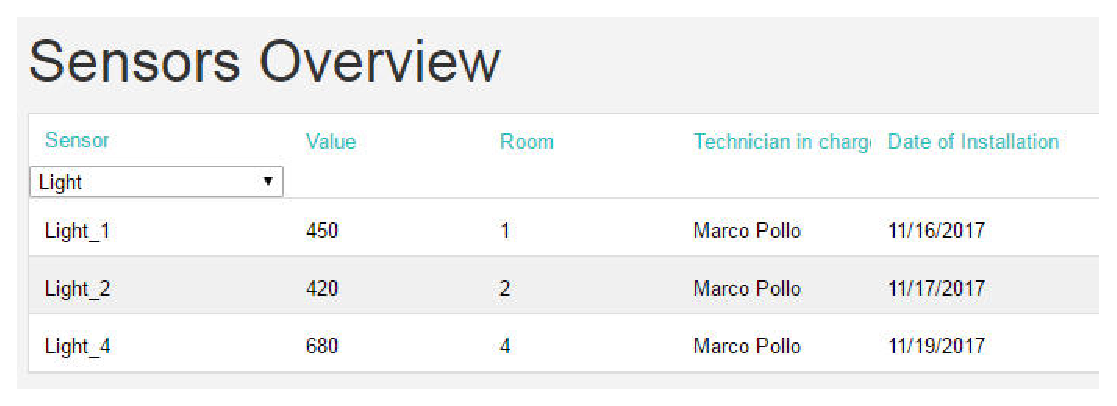
\includegraphics[width=1\textwidth]{images/LightSensor.eps}
\end{figure}
\end{enumerate}
\end{description}

\subsection{Example of humidity sensor sending digital signal}
\textbf{Light sensor 1} sends 550 nm as digital signal. \textbf{System}
updates the sensor table value from room 1 and updates the light value to 550nm.
\hfill
\vspace{0.5cm}
\hrule


\section{Motion sensor push information}

\hrule
\hfill
\vspace{0.5cm}
\label{operation:Motion sensor push information}

The Motion Sensor pushes the information to the sensor table.
\begin{description}
\item \textbf{Parameters:} \
\item \textbf{Precondition:} The system is bootedup with the respected
configurations.
\item \textbf{Post-condition:} The system sends alert to the manager.

\item \textbf{Triggering:}
\begin{enumerate}
\item \textbf{Motion sensor} sends digital signal to the system if any movement
is detected.
\item System displays an alert to the manager that there might be an intrusion.
\end{enumerate}
\end{description}

\subsection{Example of Motion sensor sending digital signal}
\textbf{Motion sensor 1} sends a digital signal to the system. The system alerts
the manager of an intrusion.
\hfill
\vspace{0.5cm}
\hrule

\break



\section{Turn on Heater}

\hrule
\hfill
\vspace{0.5cm}
\label{operation:Turn on heater}

In case the Temeprature sensor sends an a value less then 15 degrees the heater
is switched on.
\begin{description}
\item \textbf{Parameters:} temperatureOfSensor
\item \textbf{Precondition:} The system is bootedup with the respected
configurations and digital signals comming from the Temperature sensor which is
less then 15 degrees.
\item \textbf{Post-condition:} Heater in a given room is on until the
Temperature sensor sends value heigher than 19.

\item \textbf{Triggering:}
\begin{enumerate}
\item \textbf{Temperature sensor} sends digital signal of 14 to the system.
\item System enables the heater for the given room.
\item \item \begin{figure}[H]
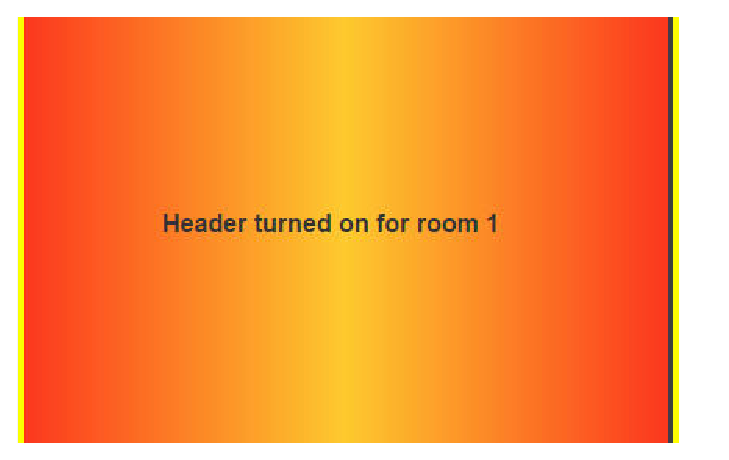
\includegraphics[width=1\textwidth]{images/TurnOnHeater.eps}
\end{figure}
\end{enumerate}
\end{description}

\subsection{Example of humidity sensor sending digital signal}
\textbf{Temperature sensor 1} sends 14 as digital signal. \textbf{System}
enables the heater to heat the room1 until the temperature sensor sends a value
heigher than 18.
\hfill
\vspace{0.5cm}
\hrule


\section{Turn on LED}

\hrule
\hfill
\vspace{0.5cm}
\label{operation:Turn on LED}

Incase the light sensor pushes a value less than 400 the LEDs qre turned on.
\begin{description}
\item \textbf{Parameters:} lightValue,timeTicker
\item \textbf{Precondition:} The system is bootedup with the respected
configurations and digital signals comming from the Lightsensor has to be less
than 400 nm and the ticker has to be 0.
\item \textbf{Post-condition:} The LEDS for the given room are turned on until
the outside Lightsensor gives a value more than 400.

\item \textbf{Triggering:}
\begin{enumerate}
\item \textbf{Light sensor} sends digital signal of less than 400 nm to the
system.
\item System enables the LEDs for the given room if the TimeTicker is 0.
\item \begin{figure}[H]
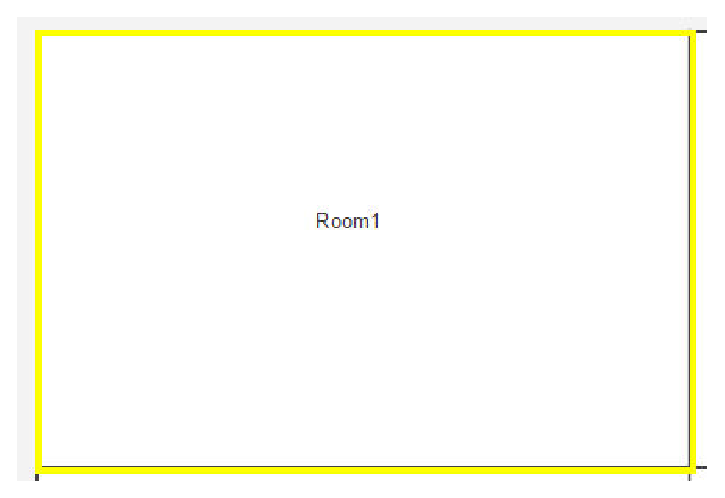
\includegraphics[width=1\textwidth]{images/LEDSON.eps}
\end{figure}
\end{enumerate}
\end{description}

\subsection{Example of humidity sensor sending digital signal}
\textbf{Light sensor 1} sends 399 as digital signal. \textbf{System}
evaluates if the timeTicker is 0 if it is it turns the LEDs on.
\hfill
\vspace{0.5cm}
\hrule




\break




\section{Open Windows}

\hrule
\hfill
\vspace{0.5cm}
\label{operation:Open Windows}

Incase the temperature sensor inside has a value higher than the value allowed.
\begin{description}
\item \textbf{Parameters:} Temperature,room,TemperatureSHouldBE
\item \textbf{Precondition:} The system is bootedup with the respected
configurations and digital signals comming from the Temperature sensor has to be
more than a given value.
\item \textbf{Post-condition:} The Windows for that given room are opend.

\item \textbf{Triggering:}
\begin{enumerate}
\item \textbf{Temperature sensor} sends digital signal of more than a given
value degrees to the system.
\item System opens the windows unitl the temperature decreeces to the requested
temperature.
\end{enumerate}
\end{description}

\subsection{Example of humidity sensor sending digital signal}
\textbf{Temperature sensor 1} sends 45 (degree) as digital signal.
\textbf{System} checks if the temperature is acceding the temperature should be
than the windows are opening.
\item \begin{figure}[H]
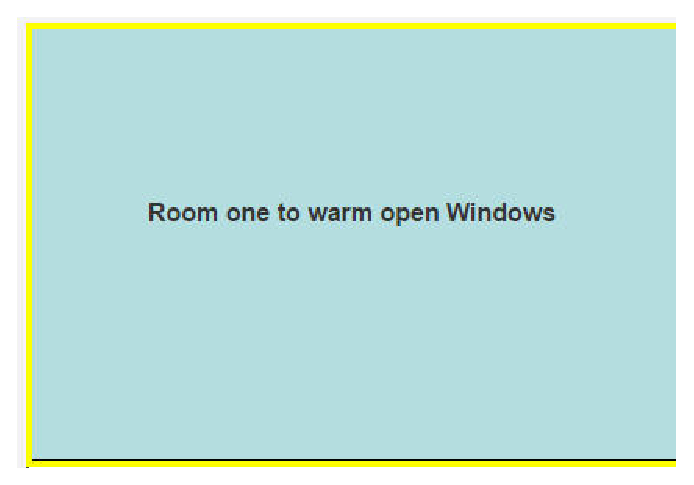
\includegraphics[width=1\textwidth]{images/OpenWindows.eps}
\end{figure}
\hfill
\vspace{0.5cm}
\hrule









\section{Turn on watering}

\hrule
\hfill
\vspace{0.5cm}
\label{operation:Turn on watering}

Incase the humidty sensor gives a value below the requested value watering is
turned on.
\begin{description}
\item \textbf{Parameters:} humidityLevel,Room
\item \textbf{Precondition:} The system is bootedup with the respected
configurations and digital signals comming from the humidty sensor has to be
less than a given level.
\item \textbf{Post-condition:} The watering is turned on for the given room.

\item \textbf{Triggering:}
\begin{enumerate}
\item \textbf{Humidty sensor} sends digital signal of less than the accepted
amount to the system.
\item System enables the watering for a given room until the humidty level is
as the room humidtyi accepts it.
\end{enumerate}
\end{description}

\subsection{Example of Enabling wateringl}
\textbf{Humidity sensor 1} sends a value of 10 since the humidity sensor is in
room1.
\textbf{System} enables the watering for the room1 until the humidity level is
40 so that the plants have enough water.
\item \begin{figure}[H]
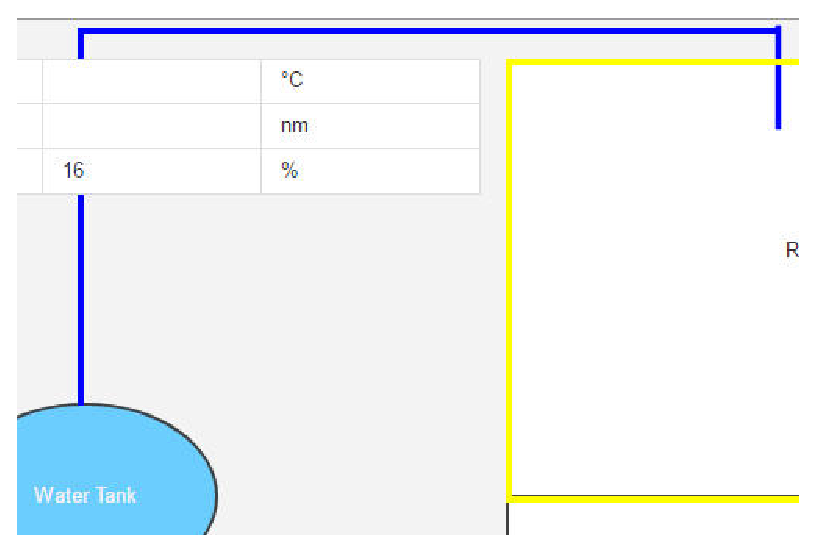
\includegraphics[width=1\textwidth]{images/WateringOn.eps}
\end{figure}
\hfill
\vspace{0.5cm}
\hrule


\break

\section{Refill storage}

\hrule
\hfill
\vspace{0.5cm}

\label{operation:Refill storage System request}

The Manager accept to refill the storage of seed requested by the system.
\begin{description}
\item
\textbf{Parameters:}Name,Amount,ph-Amount,Vegtable(boolean),TemperaturePreference
\item \textbf{Precondition:} The system is bootedup and the Manager has to be
logged in and be on the Manager request screen and there needs to be a request
from the system for seeds.
\item \textbf{Post-condition:} The inventory storage of the requested seed has
been updated.
\item 
\item \item \textbf{Output messages:} Successfully refilled the storage
\item \textbf{Triggering:}
\begin{enumerate}
\item \textbf{Manager} presses the green button on the request seed table.
\item \textbf{System} displays a message that the storage was sucessfully
refilled.
\end{enumerate}
\end{description}

\subsection{Example of accepting a request}
\textbf{Manager} Presses on the green button from Apple where the amount of
requested seeds is 20. \textbf{System} updates the inventory by adding 20 to the
apple seeds amount and displays the message: Successfully refilled storage.
\hfill
\vspace{0.5cm}
\hrule



\newpage
  
% Error messages and problem resolution

\chapter{Error messages and problem resolutions}
\label{chap:error_messages}

All known problems are listed here below with the given error codes and how to
solve them. In case an error is not listed here below please fill free to
contact us \hyperref[sec:Contact]{Click on me}.


\section{\textbf{\textcolor{red}{Error message 1}}}
\hrule
\vspace{0.5cm}
\textbf{Ph value is not correct (1)}
\subsection{Problem identification}
Ph value is defined on a scale of 1 to 14.  Where 1 is most acidic and 14 most
basic or alkaline.

\subsection{Probable cause}

The problem is due to the constraints on the Ph value text field that means the
value entred here has to be between 1 and 14.

\subsection{Corrective actions}
Enter a valid number between 1 and 14.
\vspace{0.5cm}
\hrule


\break

\section{\textbf{\textcolor{red}{Error message 2}}}
\hrule
\vspace{0.5cm}
\textbf{Crop Name not valid (2)}
\subsection{Problem identification}
The name text field input was not valid.

\subsection{Probable cause}
Due to the constraints on the Name textfield the error happens.

\subsection{Corrective actions}
The name has to be at least 5 caracters long.
\vspace{0.5cm}
\hrule
\hfill
\section{\textbf{\textcolor{red}{Error message 3}}}
\hrule
\vspace{0.5cm}
\textbf{Amount no valid input (3)}
\subsection{Problem identification}
The amount text field input was not valid.

\subsection{Probable cause}
Due to the constraints on the amount input the error happend.

\subsection{Corrective actions}
To solve the Error 3 you have to enter an amount which is higher than 0.
\vspace{0.5cm}
\hrule
\break

\section{\textbf{\textcolor{red}{Error message 4}}}
\hrule
\vspace{0.5cm}
\textbf{Temperature Prefernce is not valid (4)}

\subsection{Problem identification}
The entered text field input was not valid.

\subsection{Probable cause}
Due to the constraints on the Temperature Preference input the error happend.

\subsection{Corrective actions}
To solve the Error 4 you have to enter on the Temperature Preference a value
between 15 and 40 degrees.
\vspace{0.5cm}
\hrule
\hfill
\section{\textbf{\textcolor{red}{Error message 5}}}
\hrule
\vspace{0.5cm}
\textbf{Sensor Name not valid (5)}
\subsection{Problem identification}
The input of text field Name is not valid.

\subsection{Probable cause}
Due to the constraints on  input of Sensor Name text field the error happend.

\subsection{Corrective actions}
To solve the Error 5 you have to enter on the Sensor Name Preference a Number at
the end of the input. For good pratice use the Room number where you want to add
it as last index of the sensor name.
\vspace{0.5cm}
\hrule
\break

\section{\textbf{\textcolor{red}{Error message 6}}}
\hrule
\vspace{0.5cm}
\textbf{Room input text is not valid (6)}
\subsection{Problem identification}
The cause of the error occurs due the non valid input on the Room text field
input.

\subsection{Probable cause}
Due to the constraints on the on the input the error happens.

\subsection{Corrective actions}
To solve the Error 6 trouble you have to input on the text field Room a number
which is higher than 0.
\vspace{0.5cm}
\hrule
\hfill
\section{\textbf{\textcolor{red}{Error message 7}}}
\hrule
\vspace{0.5cm}
\textbf{Technician name is not valid (7)}

\subsection{Problem identification}
The cause of the error is due to an non valid input on the Name text field.

\subsection{Probable cause}
Due to the constraints on the input field name the error happens.

\subsection{Corrective actions}
To solve the Error 7 you have to input on the name text field a name which has
no numbers.

\vspace{0.5cm}
\hrule
\break

\section{\textbf{\textcolor{red}{Error message 8}}}
\hrule
\vspace{0.5cm}
\textbf{Reason is not valid (8)}
\subsection{Problem identification}
The cause of the error is due to a non valid input on the Reason text field.

\subsection{Probable cause}
Due to the constraints on the input field Reason the error happens.

\subsection{Corrective actions}
To solve the Error 8 you have to enter at least a 4 digit long input on the text
field Reason.

\vspace{0.5cm}
\hrule


\section{{\textcolor{red}{Error message 9}}}
\hrule
\vspace{0.5cm}
\textbf{Deletion was declined (9)}

\subsection{Problem identification}
The manager tries to decline a request.

\subsection{Probable cause}
Due to the constrain on the button after pressing it.

\subsection{Corrective actions}
To solve the Error 9 you can not delet a request where the value is 0. 0 means
there is no request at the moment.

\vspace{0.5cm}
\hrule
\break

\section{{\textcolor{red}{Error message 10}}}
\hrule
\vspace{0.5cm}
\textbf{Retriving Failed (10)}

\subsection{Problem identification}
Retriving modify on the crops inventory failed the input amount is the issue.

\subsection{Probable cause}
Due to the constraint on the amount text field the error happens.

\subsection{Corrective actions}
To solve the Error 10 you need to input an amount which is less or equal the
amount left of crops for the given crop which you want to retrive.

\vspace{0.5cm}
\hrule







\newpage

%APPENDICES
\appendix
\chapter{Greenhouse Software}
\label{chap:appendix_AllUser}


\section{Login}
\label{sec:appendix_SignIn}
\begin{figure}
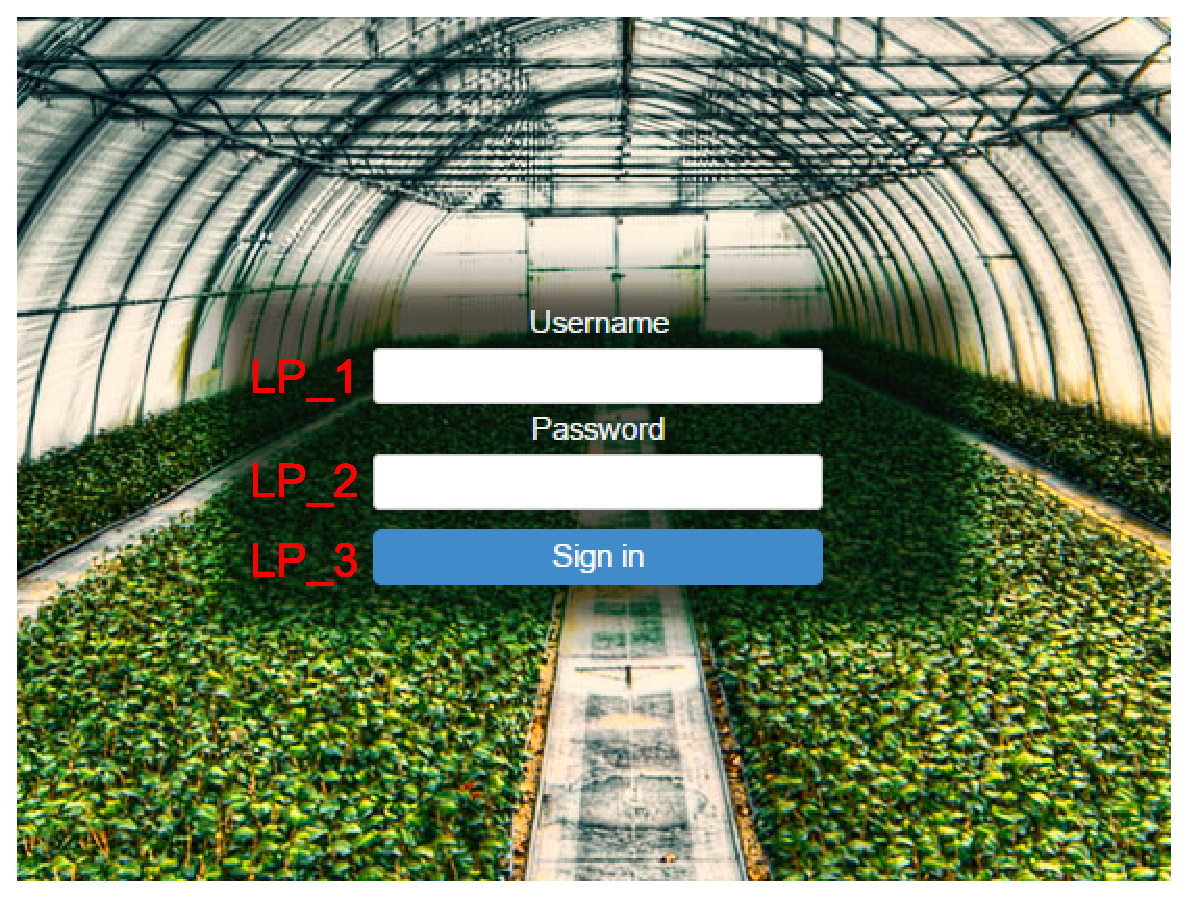
\includegraphics[width=1\textwidth]{images/appendix_images/SignIn.eps}
\end{figure}

The 'Login' page is the first page everyone sees before being able to use any
features of our software.

The User needs to identify himself with valid credentials.

\subsection{Username (LP 1)}
This input field is used for the \emph{Username} of the Gardener, Technician or
Manager.

\subsection{Password (LP 2)}
This input field is used for the \emph{Password} of the Gardener, Technician, or
Manager.

\subsection{Sign In Button (LP 3)}
This button send the request to be signed in, by clicking it.

\subsubsection{Success Scenario}
The \emph{User} is taken the \emph{Home} screen.

\subsubsection{Failure Scenario}
The \emph{User} gets a visible error message.





\newpage
\section{Home}
\label{sec:appendix_Home}
\mbox{} \par
\noindent\centerimg[width=1\paperwidth]{images/appendix_images/Home.eps}

The \emph{Home} page is the first page the \emph{User} sees after signing in.

This page gives a quick summary of the most important information about the most
recent alerts and warning, the next upcoming tasks and planned watering for each
room and low running stock. 

Further accesses through the blue and white buttons.

\subsection{Schedule (HO 1)}
The \emph{Schedule} shows a summary of the 6 next upcoming tasks of the
gardeners. The list contains information about the \emph{Date}, the \emph{Task
name}, the concerned \emph{Room} and \emph{Gardener} and a checkbox indicating
whether the task is \emph{Important}.

\subsection{Alerts and Warnings (HO 2)}
The \emph{Alerts and Warnings} list shows a summary of the 6 latest Alerts and
Warnings for the \emph{Technician}. The list contains information about the
\emph{Date} and \emph{Time} the alert or warning was added to the system, the
concerned \emph{Room} and \emph{Sensor} if there is a sensor assigned to the
alert or warning. The \emph{Error Type} gives more precise information about the
malfunctioning if it an alert. For Warnings is describes the Problem.
Additionally we get Information about the assigned \emph{Technician} if assigned
and if the problem is already \emph{Solved}.

\subsection{Storage (HO 3)}
The \emph{Storage} list shows a summary of the 6 items with the lowest quantity.
The list contains information about the \emph{Name} of the items, the current
\emph{Amount}. The other information about the \emph{pH-Amount, Vegetable and
TemperaturePref} are used to distinguish between more types of the same plant.

\subsection{Projections (HO 4)}
The \emph{Projections} grid shows a summary of the 4 next rooms planned
to be watered. The single grid contains informations about the concerned
\emph{Room} and the \emph{Date} for the next planned watering.

\subsection{View entire Schedule Button (HO 5)}
The \emph{View entire Schedule} button is a shortcut from the menu
\emph{Schedule} button. The button is designed for a fast access and has a blue
color.

\subsection{View all Alerst and Warnings Button (HO 6)}
The \emph{View all Alerts and Warnings} button is a shortcut from the menu
\emph{Alerts and Projections} button. The button is designed for a fast access
and has a blue color.

\subsection{Manage Storage Button (HO 7)}
The \emph{Manage Storage} button is a shortcut from the menu
\emph{Manager} button. The button is designed for a fast access and has a blue
color.

\subsection{View all Projections Button (HO 8)}
The \emph{View all Projections} button is a shortcut from the menu
\emph{Alerts and Projections} button. The button is designed for a fast access
and has a blue color.

\subsection{Settings Button (HO 9)}
The \emph{Settings} button opens a pop-up window with the \emph{Settings}
screen.

\subsection{View Security Camera Button (HO 10)}
The \emph{View Security Camera} button opens a pop-up window with the
\emph{Security Camera} screen.

\subsection{Exit Button (HO 11)}
The \emph{Exit} button signs the current \emph{User} out and closes the
\emph{Greenhouse} Software application.


\newpage
\section{Statistics}
\label{sec:appendix_Statistics}
\mbox{} \par
\noindent\centerimg[width=\paperwidth]{images/appendix_images/Statistics.eps}

The 'Statistics' page is the  page you see when you navigate to the Statistics
inside the menu. This page helps the operator to see more details and identify
possible problems.

\subsection{Temperature diagram (ST 1)}
The diagram represents the temperature over the last 10 days from the selected
room \textbf{(ST 1.1)}

\subsection{Water Consumption vs Luminosity Level diagram (ST 2)}
The diagram represents the water consumption with the spectral power over 
the last 10 days from the selected room \textbf{(ST 2.1)}

\subsection{Crops statistics (ST 3)}
The crops statistics help the user compare different crops that were harvested and entered into the system.
The compare checkbox \textbf{(ST 3.2)} allows the \emph{User} to select the
panel inside which the crops is loaded.

\subsubsection{Manage button (ST 3.1)}
The 'Manage' button open the Manage crops statistics. This page is only accessible as a \emph{Manager}.


\subsection{Current Stock (ST 4)}
The bar diagram represents the current available stock on seeds.





\newpage
\section{Alerts and Projections}
\label{sec:appendix_AlertsPrejections}
\mbox{} \par
\noindent\centerimg[width=\paperwidth]{images/appendix_images/AlertsProjections.eps}

The 'Alerts and Projections' page is the  page you see when you navigate to the
Alerts and Projections inside the menu. This page helps you to see the current
state of your garden.

\subsection{Alerts Database (AP 1)}
The shown table represents all the lastest alerts and warnings created by the
system. By clicking on the solved checkbox you can mark a warning as solved.

\subsection{Next Watering (AP 2)}
The shown table represents the date of the next watering for each room inside
the database of your system.

\subsection{Next Harvest (AP 3)}
The shown table represents the date of the next harvest for each room inside
the database of your system. These dates are guidelines and your plants may need
more days to be ripe.

\subsection{Water Tank (AP 3)}
The shown table represents the date of the day the water tanks should be
refilled to prevent running dry.






\chapter{Manager}
\label{chap:appendix_Manager}


\section{Settings}
\label{sec:appendix_Settings}
\mbox{} \par
\noindent\centerimg[width=\paperwidth]{images/appendix_images/Settings.eps}

The 'Settings' page can be reached on the 'Home' page. This page is reserved for
the Manager and can only then be accessed if the user is logged in as a manager.
Here you can manage the current Rooms and Security Camera inside the software.

\subsection{Room Input Formular (SE 1)}
The creation of a new room can be done inside this section. The Manager must
fill out all input fields to create a new room. If an input is invalid you will
receive a error message which can be lookep up in den Error section of the user
manual.

\subsection{Security Camera Input Formular (SE 2)}
The creation of a new security camera can be done inside this section. The
Manager must fill out all input fields to create a new room. If an input is
invalid you will receive a error message which can be lookep up in den Error
section of the user manual.

\subsection{Room List (SE 3)}
Here you see all current room inside the system. If you want to delete a room no
longer used, it can be deleted by using the red remove button inside the row of
the represented room.

\subsection{Security Camera List (SE 4)}
Here you see all current security cameras inside the system. If you want to
delete a security camera no longer used, it can be deleted by using the red
remove button inside the row of the represented room.


\newpage
\section{Security Camera}
\label{sec:appendix_SecurityCamera}
\mbox{} \par
\noindent\centerimg[width=\paperwidth]{images/appendix_images/SecurityCamera.eps}

The 'Security Camera' page can be reached on the 'Home' page. This page is
reserved for the Manager and can only then be accessed if the user is logged
in as a manager. Here you can look at all security cameras or a single security
camera.

\subsection{Security Camera View (CA 1)}
The grid represents the different cameras that can be shown if they are
connected.

\subsection{Camera Select List (CA 2)}
Select the camera you want to view and then use the button 'View Camera' (CA 3)

\subsection{View Camera Button (CA 3)}
The camera selected from the select list in (CA 2) will be shown in the Security
Camera View (CA 1)

\subsection{4-Camera View Button (CA 4)}
If a single camera is shown, you can use this button to show again 4 cameras at
the same time.



\newpage
\section{Crop Manager}
\label{sec:appendix_CropManager}
\mbox{} \par
\noindent\centerimg[width=\paperwidth]{images/appendix_images/CropManager.eps}

The 'Crop Manager' page can be reached on the 'Statistics' page inside the
Crops Statistics. This page is reserved for the Manager and can only then be
accessed if the user is logged in as a manager. Here you can manage all current
crops and create new crops.

\subsection{Crop Input Formular (CM 1)}
The creation of a new Crop can be done inside this section. The manager must
fill out all input fields to create a new crop inside the system. If an input is
not valid you will receive an error message which can be looked up in the Error
section of the user manual.





\section{Manager Home screen}
\label{sec:appendix_Manager_Home_Screen}

\begin{figure}[H]
\includegraphics[width=1\textwidth]{images/appendix_images/ManagerHomeRRR.eps}
\end{figure}

The Manager home screen is the screen which is dedicated for his tasks most of
his features are executed here like removing seed completly from the inventory
and adding seeds to the inventory.


\subsection{Inventory of Seeds (MH 5)}
The table with the title Inventory of Seeds,displays all the content of seeds
left in the global inventory.

\subsection{Gardener retrives from Inventory (MH 1)}
The table with the title Gardener retrives from inventory displays at which time
a given gardener has retrived a given amount of seeds.

\subsection{Delete from Inventory of seeds (MH 4)}
This red button executes a function/ future which allows to remove a selected
seed completly from the sees inventory table.

\subsection{Go to manager Request screeen (Special)}
This grey button can have 2 colors grey and red. By pressing the button the
manager gets redirected to the Manager request screen. In case the Button is red
the is a request that needs to be threated. If the button is Grey there is a
request which isn't urgent.In addition the access to this button is restricted
the button appears only if their is indeed a request.Else the functionalities
from the request screen are all disabled.

\subsection{Add seed to Inventory Of Seeds (MH 02)}
This orange button executes a function/feature which allows to add a seed to 
the Inventory of Seeds. The input formular (MH 03) has to be completed before
executing the feature .

\subsection{Input formular to add a seed/item MH 03}
This input fields are used to add the information to the inventory seed table. In addition if the input fields aren't valid an given error will be thrown.

\subsubsection{Errors 31}
Constrains are on the textfields. In case of a wrong input look up the Error
Section of the user manual.


















\section{Manager Request Screen}
\label{sec:appendix_Manager_Request_Screen}

\begin{figure}[H]
\includegraphics[width=1\textwidth]{images/appendix_images/ManagerRequestRRR.eps}
\end{figure}

The Manager Request screen is the screen which is dedicated to the request of an
Item from  Actors like the Gardener and the Technician or from the System. 


\subsection{Go to manager 1 screen (MR 01)}
This button redirects the manager to the Manager home screen.

\subsection{Ordering Seeds request by amount (MR 02)}
The manager can press the button arrow up or down for ascending or descening
order of the list.

\subsection{Accept requested seeds (MR 04 green)}
This green button allows the manager to execute a feature/function which accepts
a requested crop. 
\subsubsection{2 cases MR 04}
 
Request from the system automatically refills the the requested seeds.

Request from the Gardener the manager needs to add the requested crop by
it's own by adding a seed on the home screen.

\subsection{Decline a seed Request (MR 04 red)}
This red button allows the manager to execute a function/feature which allows
him to decline a request for a seed.

\subsubsection{Errors 33}
Error can be thrown in case the request is 0.


\subsection{Decline a Sensor Request (MR 06 red)}
This red button allows the manager to execute a function/feature which allows
him to decline a request for a sensor.
\subsection{Accept a Sensor Request (MR 06 green)}
This green button executes a function/feature that allows to accept a request
for a sensor from the technican.




\newpage
\section{Manage Gardener's Schedule}
\label{sec:appendix_ManageGardenerSchedule}
\mbox{} \par
\noindent\centerimg[width=1\paperwidth]{images/appendix_images/ManageGardenerSchedule.eps}

The \emph{Mange Gardener's Schedule} page is where the \emph{manager}
can modify the schedule of the gardener.

\subsection{Gardener's Schedule (GS 1)}
The \emph{Schedule} shows all the tasks for the gardener who is loged on. The
list contains information about the \emph{Date}, the \emph{Task name}, the concerned \emph{Room} and \emph{Gardener} and a checkbox indicating
whether the task is \emph{Important}.

\subsection{Filter by Room(GS 2)}
This \emph{Selec List} allows the \emph{Manager} to filter the table by room
name.

\subsection{Remove task (GS 3)}
This \emph{Button} allows the \emph{Manager} to remove the task in the current
line where the button is. The remove button is in every entry of the table.

\subsection{Date Textfield (GS 4)}
Into this \emph{Textfield} the \emph{Manager} enters the \emph{Date} of the task
he wants to add.

\subsection{Task Name Textfield (GS 5)}
Into this \emph{Textfield} the \emph{Manager} enters the \emph{Task Name} of the
task he wants to add.

\subsection{Room Textfield (GS 6)}
Into this \emph{Textfield} the \emph{Manager} enters the \emph{Room} in which
the taks the manager wants to add will be completed.

\subsection{Gardener Textfield (GS 7)}
Into this \emph{Textfield} the \emph{Manager} enters the \emph{Name} of the
\emph{Gardner} that will complete the task he wants to add.

\subsection{Task Description (GS 8)}
Into this \emph{Textfield} the \emph{Manager} enters the \emph{Task Description}
of the task he wants to add.

\subsection{Add Button(GS 9)}
This \emph{Button} is pressed by the \emph{Manager} when he filled out all
the textfield and selected the importance (GS 10). This will add the task to the
Gardener's schedule if all the textfields are filled out correctly.

\subsection{Importance Checkbox (GS 10)}
With this \emph{Checkbox} the \emph{Manager} chooses if the \emph{importance} of
the task he wants to add.

\subsection{Search Gardeners Schedule Textfield (GS 11)}
Into this \emph{Textfield} the \emph{Manager} can enter any information he wants
to look up in the \emph{Gardeners's Schedule}. The \emph{Manager} can search for
a \emph{Date}, \emph{Task Name}, \emph{Room}, \emph{Gardener's Name} or
\emph{Task Description}.

\subsection{Launch Search (GS 12)}
When the \emph{Manager} presses this \emph{Button} the search mention in (GS
11) will be launched.




\newpage
\section{Manage Technician's Schedule}
\label{sec:appendix_ManageTechnicianSchedule}
\mbox{} \par
\noindent\centerimg[width=1\paperwidth]{images/appendix_images/ManageTechnicianSchedule.eps}

The \emph{Mange Technician's Schedule} page is where the \emph{manager}
can modify the schedule of the technician.

\subsection{Technician's Schedule (TS 1)}
The \emph{Schedule} shows all the tasks for the technician who is loged on. The
list contains information about the \emph{Date}, the \emph{Task name}, the
concerned \emph{Room} and \emph{Technician} and a checkbox indicating whether
the task is \emph{Important}.

\subsection{Filter by Room(TS 2)}
This \emph{Selec List} allows the \emph{Manager} to filter the table by room
name.

\subsection{Remove task (TS 3)}
This \emph{Button} allows the \emph{Manager} to remove the task in the current
line where the button is. The remove button is in every entry of the table.

\subsection{Date Textfield (TS 4)}
Into this \emph{Textfield} the \emph{Manager} enters the \emph{Date} of the task
he wants to add.

\subsection{Task Name Textfield (TS 5)}
Into this \emph{Textfield} the \emph{Manager} enters the \emph{Task Name} of the
task he wants to add.

\subsection{Room Textfield (TS 6)}
Into this \emph{Textfield} the \emph{Manager} enters the \emph{Room} in which
the taks the manager wants to add will be completed.

\subsection{Technician Textfield (TS 7)}
Into this \emph{Textfield} the \emph{Manager} enters the \emph{Name} of the
\emph{Technician} that will complete the task he wants to add.

\subsection{Task Description (TS 8)}
Into this \emph{Textfield} the \emph{Manager} enters the \emph{Task Description}
of the task he wants to add.

\subsection{Add Button(TS 9)}
This \emph{Button} is pressed by the \emph{Manager} when he filled out all
the textfield and selected the importance (GS 10). This will add the task to the
Technician's schedule if all the textfields are filled out correctly.

\subsection{Importance Checkbox (TS 10)}
With this \emph{Checkbox} the \emph{Manager} chooses if the \emph{importance} of
the task he wants to add.

\subsection{Search Technician's Schedule Textfield (TS 11)}
Into this \emph{Textfield} the \emph{Manager} can enter any information he wants
to look up in the \emph{Technician's Schedule}. The \emph{Manager} can search
for a \emph{Date}, \emph{Task Name}, \emph{Room}, \emph{Technician's Name} or
\emph{Task Description}.

\subsection{Launch Search (TS 12)}
When the \emph{Manager} presses this \emph{Button} the search mention in (GS
11) will be launched.


\chapter{Technicien}
\label{chap:appendix_Technicien}



\chapter{Gardener}
\label{chap:appendix_Gardener}


	

\newpage
 
    
%GLOSSARY
%Uncomment the line below if you want to print all glossaries no matter if they
% appear in the document
%\glsaddall
\printglossaries
\newpage


%BIBLIOGRAPHY
\cleardoublepage 
\bibliographystyle{./../lu.uni.lassy.excalibur.standard.report.libraries/styles/lncs} 
\bibliography{./../lu.uni.lassy.excalibur.standard.report.libraries/defs/references/messir,doc/bibliography/user-manual}
\label{sec:references}

 
\end{document}
